\begin{spacing}{1.5}
\setcounter{chapter}{1}
\chapter{Capítulo II: \\Fundamento Teórico}
\thispagestyle{empty}

\section{Estado del Arte}
A pesar de ser un campo relativamente nuevo, la Ciencia de Datos está profundamente sustentada por la teoría académica (quizás por sus implicaciones como campo multidisciplinario y su importancia para la solución de problemas que impactan otras disciplinas).

De acuerdo a la bibliografía existente, la primera persona en hacer un bosquejo de la idea fue el académico Danés Peter Naur en su libro “Concise Survery of Computer Methods”. Naur sin embargo utiliza el término más que nada para sustituir el de ciencia computacional \cite{naur}. El investigador de Laboratorios Bell y profesor de la Universidad de Princeton, John Tukey, hace un mejor acercamiento al escribir el primer artículo científico sobre como la disciplina de la estadística cambiaba con el advenimiento de la informática \cite{tukey}. Mucho más tarde fue el estadista de la Universidad de Tokio Chikio Hayashi quien definiría de manera sucinta el concepto de Ciencia de Datos como un concepto sintético para unificar la estadística, el análisis de datos y los métodos relacionados con la consecución lo resultados \cite{hayashi}.

Es interesante que los métodos de aprendizaje automatizado proliferaron de forma paralela al concepto de ciencia de datos, y solo fueron absorbidos por esta en los últimos diez años. Alpaydim nos describe el aprendizaje automatizado como la programación de computadoras para optimizar un criterio de desempeño utilizando datos o experiencia pasada \cite{alpaydin}. Tom Mitchell respeta este concepto al describir el aprendizaje automatizado como “… la construcción de programas computacionales que aprenden con la experiencia…” \cite[pag. XV]{mitchell}. Solo Peter Harrington utiliza una descripción mucho más simplista al determinar que “El aprendizaje automatizado es la extracción de información de la data.” \cite[pag. 5]{harrington}.

La teoría detrás de la regresión lineal es bastante homogénea a través de todos los autores. Zumel y Mount describen la regresión lineal como el más común de los métodos de aprendizaje automatizado \cite{zumelMount}, y si no, es muy fácil verificar cual otro método probar como segunda opción. Para Daroczi, el énfasis está en los modelos de regresión multivariable (una extensión de la regresión lineal simple de un solo predictor y resultado) que construyen el camino para la predicción de fenómenos complejos en la naturaleza y negocios \cite{daroczi}. Por su parte, Harrington resume los beneficios de la regresión lineal \cite{harrington} por la facilidad de interpretar los resultados y lo frugal en el uso de ciclos de computación (aunque puede ser menos útil si el fenómeno no es perfectamente lineal).
 
Muchos autores han escrito sobre las series de tiempo, pero es difícil agregar al tema o discutir las ideas del profesor Robert Hyndman, uno de los expertos más respetados en la comunidad de la estadística por su trabajo en las series de tiempo. Hyndman extiende la teoría a las series de tiempo como elementos de pronóstico y su relación con la regresión lineal \cite{hyndman}. Desde el punto de vista técnico, Hyndman es el creador de varias bibliotecas de funciones de pronóstico utilizando series de tiempo y ARIMA en lenguaje R. Dentro de la bibliografía, Daroczi es quien agrega detalles sobre la detección temprana de valores atípicos que pueden dificultar – y mucho – el análisis \cite{daroczi}. Un componente importante de las series de datos es la detección de si son o no auto-regresivas (lo que determina mucho de su poder predictivo). La fórmula para la detección de series auto-regresivas es el test Dickey-Fuller, y la mejor bibliografía es el artículo científico escrito por ambos profesores en la revista especializada Econometrica (Dickey, D., y Fuller, W., 1981). A pesar de ser un artículo contemporáneo, la teoría detrás de la prueba Dickey-Fuller nos permite descartar series de tiempo no-regresivas con poco poder de predicción.
 
El uso de modelos ensamblados es en cierta forma la prueba final de la hipótesis de trabajo: la utilización de dos modelos entrecruzados cuyos resultados conforman una tabla temporal de valores esperados de los cuales se genera un nuevo modelo sintético de predicción más general y con mayor capacidad de predicción en juegos de datos de validación cruzada. Este concepto es novel; Witten y Frank lo describen como combinación de métodos múltiples, y escriben: “… un enfoque obvio para hacer mejores decisiones es tomar el resultado de diferentes métodos y combinarlos…” (Witten, I. y Frank, E., 2005). Zhou nos describe que “… los modelos ensamblados que entrenan múltiples variables y luego las combinan para uso de entrenamiento, con el Boosting y el Bagging como representantes principales, representan lo más novedoso en el estado del arte de la ciencia de datos…” (Zhou, Z., 2012, pg. VII). De una manera un tanto más coloquial, Zhang y Ma describen el uso de modelos ensamblados con una analogía de la vida real, en la cual los pacientes buscan una segunda y hasta tercera opinión de expertos antes de someterse a una operación complicada (Zhang, C. Y Ma, Y., 2012). Curiosamente tanto Zhang, Ma y Zhou hablan de la combinación de métodos de regresión general con clasificadores, y solo Witten y Frank hablan de otras combinaciones (por supuesto, Witten y Frank comenzaban a escribir en los albores del ensamblaje de métodos, cuando los clasificadores no estaban tan de moda porque el análisis era mayoritariamente de números, algo que cambió con el avance de las redes sociales).

En su libro “Crisis Cambiarias en Países Emergentes” el Dr. Bernardo Carriello utiliza un modelo de descripción (más que de predicción) de corrida de las tasas de cambios, en el cual los regresores incluían variables de medición económicos como crédito privado como porcentaje del PIB, tasa de variación de reservas, desalineación de tipo real, y otros (Carriello, B., 2010). Carriello utiliza muchísimo modelos lineales dicotómicos que modelan los escenarios con variables binarias (algo muy común entre los economistas) que por lo general favorecen regresiones logísticas o con la utilización de variables dummy o comodín (se multiplican por el coeficiente uno o cero según tengan o no valor). La mayoría de la bibliografía de aprendizaje automatizado y ciencias de datos prefieren el estudio de variables continuas y reales con amplitud de rango y valores, algo que está más cerca de la disciplina de la bioestadística que de la economía. Una pregunta adicional válida es si tomar metodologías más cercanas a la bioestadística se aplica para la predicción financiera mejor que los modelos dicotómicos actuales.
 
Volviendo a la pregunta mayor de área, el autor y antiguo Ministro de Economía de Colombia, Alfonso Ortega Cárdenas, menciona como material de bibliografía universitaria, la re-valorización del dólar frente al peso colombiano tras el comienzo de la caída de los precios del petróleo a partir del año 2015 (Cárdenas, A., 2016). El Dr. Cárdenas no hace mucho hincapié en la correlación de ambas variables, y prefiere ahondar en temas macro-económicos como la variación de la tasa de interés como elemento de presión en la tasa cambiaria y las leyes de ingreso de capital extranjero. Pero es claro que el efecto de las fuentes de ingreso del petróleo como variable clave en el valor final de la TRM ya han sido definidas – si bien algo ligeramente – como claves en un libro de texto de economía de Colombia. ¿Hay elementos adicionales que indiquen la importancia de otras fuentes de ingresos como posibles modeladores y variables de predicción de la TRM? Si los hay, y aparecen en la misma bibliografía de Cárdenas quien describe en detalle a) el sector petrolero, b) el sector siderúrgico, c) el carbón, y d) el níquel.
 
Los investigadores Mehreen Rehman, Gul Muhammad Khan y Sahibzada Ali Mahmud han utilizado la ciencia de datos para la predicción de FOREX. Los autores utilizan CGP (Programación Genética Cartesiana), una extensión del uso de redes neuronales, para obtener predicciones del dólar australiano con 98.72\% de precisión por períodos extendidos de hasta 1,000 días (Rehman, M., Khan, G. y Mahmud, S., 2014). Los autores alimentan el sistema CGP con información histórica de las monedas en cuestión compuesta por 500 días de cotización.
 
Quizás menos conocido es el uso de clasificadores versus regresores. Este camino toma el estudio de los doctores Hossein Talebi, Winsor Hoang y Marina Gavrilova. En su investigación en búsqueda de la mejora de sistemas automatizados de corretaje de FOREX utilizando aprendizaje automatizado, los autores proponen un nuevo método de clasificación. Dicho método utiliza extracción de clasificadores de múltiples escalas para el entrenamiento de datos, y luego se ensamblan diferentes clasificadores por voto Bayes (Talebi, H., Hoang, y Gavrilova, M., 2014). El método propuesto demuestra superioridad a la hora de ensamblar clasificadores por encima de clasificadores individuales.
 
Otro estudio interesante es el de los profesores de matemática de la universidad de Beijing Lean Yu, Shouyang Wang, y K. K. Lai. El enfoque es novedoso en el sentido que utilizan un sistema ensamblado de auto-regresión lineal generalizada (GLAR) con redes neuronales artificiales (ANN). Los autores llegan a la conclusión que los resultados en las predicciones son superiores a los resultados de las predicciones de los métodos por separado, o de métodos similares con regresiones lineales (Yu, L., Wang, S., Lai, K., 2005). Una lectura cuidadosa de los resultados evidencia márgenes de error del 1.56\% al 3.57\%, dependiendo de la moneda a evaluar.

\section{Marco Teórico}
La Ciencia de Datos se caracteriza por ser una ciencia multidisciplinaria. A la par de extenso conocimiento de estadística y programación, el científico de datos debe poseer un conocimiento extremo sobre el campo de acción o \textit{domain expertise} como se le conoce en inglés \cite{pengMatsui}. Este portafolio de conocimiento se refleja de igual manera en el marco teórico del trabajo de investigación, que debe unir, analizar y sintetizar la teoría de la estadística descriptiva e inferencial, el aprendizaje automatizado y los modelos ensamblados para la resolución del problema, y la economía de Colombia para entender el problema en toda su magnitud. Por tales razones se ha decidido desglosar el marco teórico en seis secciones diferentes, cada una con su base de conocimiento distintivo. 

\begin{enumerate}
    \item La Economía de Colombia
    \item Regresión Lineal
    \item Series de Tiempo
    \item La Ciencia de Datos
    \item Aprendizaje Automatizado
    \item Modelos Ensamblados
\end{enumerate}

Cada una de estas secciones se unen en un todo final para una solución holística del problema de investigación.

\section{Economía de Colombia}
Para la creación de un modelo de predicción de la TRM de Colombia, tomando como hipótesis de trabajo que existe un número finito y reducido de variables de aporte que regulan el valor de la misma a través de los ingresos por exportación y su contribución a la economía nacional, se debe primeramente comprender y definir estos conceptos. La sección del marco teórico que cubre la economía de Colombia, tiene como finalidad abarcar los siguientes temas. 

\begin{enumerate}
	\item Definir correctamente el concepto de tasa de cambio y su específico colombiano, la tasa de mercado representativa, desentrañando la formula que usa la Superintendencia Bancaria para su valuación diaria.
	\item Entender las bases del comercio internacional de Colombia y cuales son sus principales productos de exportación, sobre todo con el afán de identificar correctamente candidatos como variables de aporte para alimentar de datos el modelo de aprendizaje automatizado. 
	\item Por último, especificar el funcionamiento de los elementos financieros derivados de compra de divisas tales como los \emph{forward} y su correspondiente reglamentación bajo la leyes de Colombia. 
\end{enumerate}

Entender el funcionamiento de la economía de Colombia, sus principales componentes de exportación, y los marcos legales que rigen las estructuras de la TRM y los productos financieros de compra y venta de divisas, nos da luces no solo para entender correctamente el problema, sino para plantear propuestas de solución matemáticas que tengan una amplia correlación entre el modelo abstracto y el comportamiento en la vida real del proceso. 

\subsection{La Tasa de Cambio}
La moneda de un país tiene una equivalencia en moneda de otro y ese valor se conoce como tasa de cambio. Explicamos el concepto apoyados en los escritos del autor Mauricio Cárdenas \cite{cardenas}. También es importante explicar porqué los productos de exportación tienen un efecto en la canasta de divisas y la balanza de pagos \cite{crisisCambiarias}.   

\subsection{La TRM}
Dennis Robertson (Robertson, 1922) definió el dinero como \textit{"todo aquello generalmente aceptado para el pago de una obligación"}. El dinero en su forma más simple es el medio de pago de total liquidez, constituido por el \textit{efectivo} (billetes y monedas) y puesto en circulación por la Banca Central y por el \textit{dinero bancario}, correspondiente a los depósitos en bancos comerciales que son transferibles por medio de cheque. 

El intercambio de bienes y comercio internacional se realiza tomando como premisa que países con diferente moneda tendrán que llegar a algún tipo de mecanismo para compensar las compras, ventas y pagos de las mismas entre ambos actores. A falta de una moneda común (por lo menos en términos legales) el mecanismo que rige dicha condición de medio de operación es la tasa de cambio.

\subsubsection{Concepto: Tasa de Cambio}
Para entender el concepto de la tasa representativa de mercado, es importante primero entender el concepto de tasa de cambio. Dicha idea es muy sencilla, y gira entorno al valor de una moneda en relación con otra (Fishwick, Georgiou, Huston, y Marechal, 2010). En épocas pasadas, el tipo de cambio era fijo, pero esta teoría ha quedado atrás con la implementación de tipos de cambio de flotación libre. La preocupación de los gobiernos gira en procurar mantener un determinado tipo de cambio ni estimule la revalorización de la moneda, ni mucho menos genere una devaluación de la misma (Cárdenas, 2016). 

\subsubsection{Devaluación de la Moneda} 
Se entiende como devaluación monetaria la pérdida del valor nominal de la moneda nacional frente a otra u otras monedas extranjeras. Las causas generadoras de la devaluación se pueden sintetizar principalmente en dos:

\begin{itemize}
	\item Falta o disminución de la demanda de la moneda nacional.
	\item Una mayor demanda de la moneda extranjera por parte de los consumidores y comerciantes de la nación.
\end{itemize}

En un sistema de cambio libre (dólar de flotación), en el cual la intervención del Banco de la República es nula, la devaluación toma el nombre de \textit{depreciación}. 

\subsubsection{Apreciación de la Moneda Local}
A veces, por causas externas a la economía de un país, la moneda local se ve sobrevaluada, sea por la abundancia de dólares procedentes del exterior o por el ingreso de capitales extranjeros al país. Esto genera que haya más reservas de dólares, provocando que la moneda local se aprecie por la mayor oferta de los capitales extranjeros. 

\subsubsection{Dólar de Flotación}
El 25 de septiembre de 1999, la Junta Directiva del Banco de la República de Colombia optó por desmontar la banda cambiaría y dar paso al dólar flotante. Cuando el precio de la divisa se mueve por libre juego de la oferta y la demanda, sin límite de techos o pisos, se habla de un régimen de flotación. La flotación implica que el Banco de la República no tendrá en adelante ninguna injerencia en la fijación del precio del dólar (Cárdenas, 2016). 

Las oportunidades en las cuales el estado ha tratado de varias formas de estabilizar la moneda y el tipo de cambio no han sido pocas. El país ha pasado a través de ciclos de revaluación y devaluación alternados, ambos con impactos negativos para la economía. 

\begin{enumerate}
	\item En el año 2007 el Gobierno Nacional intentó frenar el ingreso de dólares producto de capital golondrina con medidas de cautelas de depósitos de un cuarenta por ciento del valor durante seis meses, tratando de evitar la especulación (Decreto 2466 MINHACIENDA, Junio 2007)
	\item La disminución de los capitales y el aumento del desempleo llevó al Gobierno Nacional a desarticular dicha medida en el año 2008 (Decreto 1888 MINHACIENDA, Mayo 2008)
	\item En el año 2012 el Banco de la República tomo la estrategia de compras diarias de treinta millones de dólares como forma de mantener la moneda estable y lejos de la apreciación (Empresarios piden bajar tasas de interés por caída del dólar. (Enero 27 del 2012) Portafolio, pp.3)
	\item Hacia el año 2014 el Banco de la República, habiendo conseguido su meta de una tasa de cambio estable, redujo notablemente sus esfuerzos de compras de la divisa americana. Lamentablemente hacia mediados del 2015, la caida de los precios del petroleo tuvo un efecto nefasto en la devaluación del peso colombiano, que llegaría a tasas de cambio a finales del año cercanas a los \$3,300 pesos. 
\end{enumerate}

\subsubsection{La TRM (Tasa Representativa del Mercado}
La Superintendencia Financiera de Colombia es la que calcula y certifica diariamente la TRM con base en las operaciones registradas el día hábil inmediatamente  anterior  y  la  define  de  la  siguiente  manera  (Circular  Reglamentaria Externa del Banco de la República DODM-146, 2015):

	\begin{quote}La  tasa  de  cambio  representativa  del  mercado  (TRM)  es  la  cantidad de pesos colombianos por un dólar de los Estados Unidos (antes del 27 de noviembre de 1991 la tasa de cambio del mercado colombiano estaba dada por el valor de un certificado de cambio). La TRM se calcula con base en las operaciones de compra y venta de divisas entre intermediarios financie-ros que transan en el mercado cambiario colombiano, con cumplimiento el mismo día cuando se realiza la negociación de las divisas.
	\end{quote}

La Superintendencia Financiera de Colombia no determina el valor de la TRM sino de un elemento derivado de las operaciones de compra y venta de la misma. Son los agentes de operación (exportadores que venden sus productos en dólares y los deben canjear a pesos colombianos e importadores que compran sus productos en dólares y para tal fin cambian sus pesos colombianos). Ambos obedecen a fuerzas del mercado que dan forma y materializan la valorización.

\subsection{Exportaciones de Colombia}
Si bien no buscamos ser expertos en ninguno de los tipos de exportación que hace Colombia, es importante en esta sección describir uno a uno los rubros con mayor contribución, ya que serán nuestras variables independientes para aplicar en el proceso de aprendizaje automatizado y modelar el comportamiento futuro de la TRM. 

\subsubsection{El Petróleo}
Del petróleo se dice que es el energético más importante en la historia de la humanidad, que es un recurso no renovable que aporta el mayor porcentaje del total de la energía que se consume en el mundo. En cuanto a Colombia, hace parte del grupo de países en el mundo que tiene petróleo, sin llegar a ser un país petrolero; su producción para el año 2015 tan solo alcanzó un millón de barriles diarios, de los cuales no todos son clasificados como los mejores, ya que no alcanzan según las normas API el nivel superior a 26 grados (Cárdenas, 2016). 

En Colombia los recursos naturales no renovables, entre ellos, los hidrocarburos, son propiedad del Estado. La política petrolera es definida por el Gobierno Nacional a través del Ministerio de Minas y Energía, y hasta el año 2003 Ecopetrol era la empresa encargada de su ejecución. 

\subsubsection{El Carbón}
Colombia, en cuanto a recursos carboníferos se refiere, ocupa dentro de los países latinoamericanos un lugar privilegiado, pues cuenta con las mayores reservas y cuenta con gran variedad de calidades. Este potencial carbonífero está distribuido en las tres cordilleras principales, correspondiendo la mayor parte a la cordillera oriental \cite{cardenas}. Colombia es el país con mayores reservas de carbón en América Latina, cuenta con recursos potenciales de 16,992 millones de toneladas (MT) de los cuales 7,063 MT son medidas, 4,571 MT son indicadas, 4,237 MT son inferidas y 1,119 MT son recursos hipotéticos. Por otra parte, es el sexto exportador de carbón del mundo, con una participación de 6,3\%, equivalente a 50 MT anuales de carbón \cite{carbonMain}. 

La importancia del carbón colombiano, más que por sus características, es por su posición estratégica (particularmente en las minas de la Guajira), pues facilita el acceso al mercado europeo y norteamericano, y porque ha logrado, con relativo éxito, la conquista de dichos mercados por su precio y calidad respecto al de los carbones procedentes de Australia e Indonesia \cite{cardenas}. Con la tasa de explotación actual, las reservas medidas de carbón en Colombia aseguran más de 120 años de producción, suficientes para participar a gran escala en el mercado internacional y abastecer la demanda interna \cite{carbonMain}

El carbón, fuente generadora de divisas y de empleo, concentra el 47\% de la actividad minera nacional y representa el 1\% del producto interno bruto colombiano con algo más de 3,4 billones de pesos \cite{carbonMain}. En los últimos años se ha consolidado en el segundo producto de exportación nacional  después del petróleo y se estima que bajo las condiciones de mercado actuales, entre el 2010 y 2015 podría superar las exportaciones de petróleo.

\subsubsection{El Café}
El café es uno de los productos básicos del mundo que más se comercia. Es el principal producto agrícola de Colombia, y de él depende un porcentaje significativo de la economía y el sustento de gran parte de la población. El café Colombiano es reconocido a nivel mundial a través de su marca registrada Juan Valdez. Dado que es una de las exportaciones que continua creciendo, es de esperar que sea una fuente de divisas y exista una correlación estrecha entre el precio del café y el valor de la TRM. 

Se cree que los Jesuitas fueron los primeros en cultivar café en Colombia en la región del Orinoco, hacia 1732. Posteriormente, difundieron su cultivo por el sur del país. El párroco de Sálazar de las Palmas, Francisco Romero, ferviente admirador de la planta, impuso como penitencia a sus feligreses la siembra de cafetos según la gravedad de los pecados. Su ejemplo, seguido por otros sacerdotes y así se propagó el café por el nororiente del país. A mediados del siglo XIX el cultivo del café se expandió del norte al centro y occidente del territorio.A finales de ese siglo, se consolidó como cultivo de exportación. Desde cuando comenzaron a tener forma ordenada el cultivo y la actividad exportadora de café en Colombia, el producto ha estado estrechamente ligado al desarrollo y bienestar del país \cite{cafeMain}.

Actualmente, el café genera más de 1 millón de empleos permanentes de los cuales 800,000 se ocupan de las labores agrícolas. Más de 500,000 familias se benefician de su cultivo. Todos los cafetales sembrados hasta 1993 estaban en producción y las exportaciones ascendieron a cerca de 532,000 sacos. Para mediados de la década de los 90, el café representaba mucho más de la mitad del valor total de las exportaciones colombianas, y en los años pico de 1995 y 1996 el café significó cerca del 70 por ciento del valor total delas exportaciones. Alrededor de 1 millón de hectáreas están sembradas en café, lo que equivale al uno por ciento del área total de Colombia. Las zonas cafeteras se distribuyen a lo largo de las pendientes de las cordilleras en un microambiente especial de clima templado. La mayor cantidad de cultivos se encuentra en los departamentos de Antioquia, Caldas, Risaralda, Quindío, Tolima y Valle del Cauca \cite{cafeMain}

Colombia tiene, pues, gran tradición como país productor y exportador de café. La actividad cafetera favoreció el aumento y la expansión de la industria manufacturera, el crecimiento de las ciudades, el desarrollo de la infraestructura de transporte, la formación del sector financiero y la vinculación del país al comercio internacional.

\subsubsection{El Níquel}
El  desarrollo  de  la  minería  en  Colombia, aún en proceso de mejoramiento, muestra el adelanto de la industria del Níquel como una de las que mayores beneficios le han dado  al  país,  al  lado  de  los  grandes  progresos que se tienen en el sector carbonífero, siendo estas por excelencia las exportaciones tradicionales del país, en lo que compete al sector minero, con el petróleo y carbón \cite{niquelMain}.

La importancia del níquel radica en las aleaciones con otros elementos para dar fuerza y resistencia a la corrosión en amplias variaciones de temperatura. Se utiliza principalmente en aleaciones con el hierro y el acero para las fabricaciones de aceros inoxidables empleados en la industria en forma general. En Colombia, los recursos identificados pertenecen al grupo de las lateritas niquelíferas, producto de la alteración de las rocas ultramáficas del conocido sistema tectónico ofiolítico \cite{cardenas}.

En Colombia existen seis yacimientos de Níquel, tres de ellos están localizados en la región Caribe, en el departamento de Córdoba (Cerro Matoso, Planeta Rica  y Uré). Los tres restantes se encuentran en el departamento de Antioquia (Ituango, Morro Pelón y Medellín) \cite{niquelMain}.

Cerro Matoso es una mina de extracción de Níquel integrada con el proceso de  fundición, que además combina los depósitos lateríticos de Níquel más ricos del mundo, con una fundición de Ferroníquel a bajo costo, lo cual la ha convertido en uno de los productores de Ferroníquel con más bajo costo de producción en el mundo \cite{niquelMain}.

Colombia es el primer productor de Níquel en Suramérica y el tercero en Centroamérica y el Caribe, después de Cuba y República Dominicana. Cerro Matoso aporta el 10\% de la producción mundial de Ferroníquel y un 3\% de la producción mundial de Níquel. La producción industrial se hace en lingotes de Ferroníquel con un contenido de 37,5\% de Níquel \cite{niquelMain}.

\subsubsection{El Oro}
De acuerdo a la Contraloría General de la República,se afirma que en Colombia hay 17 departamentos y 80 municipios donde se llevan a cabo procesos de extracción artesanal, pequeña o industrial de oro y según la UPME, Antioquía y   Bolívar poseen la mayor cantidad de minas del país y producen alrededor de  18.8  MT de oro anuales, si bien departamentos como Chocó, Córdoba, Caldas y Tolima  también tienen amplia presencia de la actividad extractiva del metal \cite{oroMain}.

La actividad de extracción del oro en el país se podría nominar como atomizada, es decir, existen múltiples actividades de extracción en diferentes zonas, la mayoría de las cuales no cuenta con una legalidad o formalización en su actividad. Tomando datos oficiales, existen 4,133 unidades de minería que son  equivalentes al 29\% de la minería con o sin título minero, de las cuales 3,584 son ilegales. Esto representa el 40\% del total de la ilegalidad de minería en el país, lo cual indica que de cada cinco unidades ilegales dos pertenecen al oro \cite{oroMain}. 

Lamentablemente la explotación del oro tiene una connotación negativa en el país. La Dra. Adriana Arango nos ilustra \cite{arango_2017}:

\begin{quote}
Después de la independencia de Colombia, el oro pasó a ser propiedad de la Nación y desde entonces la minería se convirtió en un sector económico regulado por la legislación nacional. Luego de muchos años de explotación, mayormente por la industria, medianos y pequeños mineros, los grupos armados pasaron a tomar parte en el negocio de la minería de oro, ya sea extorsionando mineros y/o extrayendo oro de forma ilegal. Esto ocurrió a partir de las negociaciones formales de paz entre el gobierno y la guerrilla en 2012, donde el oro se convirtió en una actividad económica que sostenía las organizaciones armadas. A pesar de que los grupos insurgentes (FARC y ELN) estaban adquiriendo un promedio de \$600 millones al año, proveniente del negocio de cultivos ilícitos, extorsión, secuestro, ganado robado, y otras fuentes; el oro también se volvió lucrativo debido a su pequeño volumen y su alto valor. El incremento de explotación de oro por parte de grupos armados incrementó con el aumento en el control de cultivos ilícitos en el país. Así, la extracción de oro pasó de 47.8 MT en 2009 a 66.2 MT en 2012, cifra que se ha mantenido hasta el 2016.
\end{quote}

Es interesante que los ingresos por la extracción del oro pasan en gran parte por la economía informal. ¿Cuál es el impacto de ingresos informales del oro en la tasa de cambio del dólar en Colombia? Si bien esta no es una pregunta que nos hacemos en el proyecto de investigación, se podrá contestar cuando se mida el coeficiente de determinación y el coeficiente de correlación de Pearson en el capítulo 4 de análisis y discusión de resultados.  

\subsubsection{El Banano}
El banano es el cultivo que ocupa el primer lugar en las exportaciones agropecuarias menores. Las principales zonas de cultivo son las de Urabá (72\% de la producción) y Santa Marta. Los principales problemas en el cultivo son las plagas, los problemas socio laborales, los vientos huracanados y problemas internacionales por la aparición de otros tipos de banano de mejor aceptación. Aunque el volumen de producción de Colombia se ve superado por Ecuador, existen óptimas condiciones para la producción a bajos costos. La fruta es cultivada desde el nivel del mar hasta alturas de 2,200 metros. El consumo nacional ha mejorado y cada vez se han ido extendiendo los cultivos en algunas fincas del Quindío y del Valle del Cauca, intercalando con el plátano \cite{bananoC}.

Colombia ha tenido una relativa larga tradición como productora y exportadora neta de banano de exportación tipo \emph{Cavendish Valery}. La agroindustria bananera se ha desarrollado como una cadena agroexportadora tradicional, generando importantes divisas para el país, manteniendo su posición como exportadora neta, después del café y las flores. En el país existen dos tipos de banano: el banano de exportación y el banano criollo o de consumo interno \cite{bananoFINAGRO}.

\begin{itemize}
\item El banano de exportación: las regiones del Golfo de Urabá y el nororiente del departamento del Magdalena, se han especializado en la producción y exportación de banano y plátano con altos niveles de productividad e integración de los productores y comercializadores, gracias a las ventajas comparativas de localización y calidad de los suelos con respecto a otras zonas productoras del mundo.
\item El Banano Criollo: El banano criollo (común y murrapo) o de consumo interno, según datos del Ministerio de Agricultura, se produce principalmente en el Valle del Cauca, Tolima y Antioquia y tiene un área cosechada y una producción significativamente menores al de exportación.
\end{itemize}

La Asociación De Bananeros De Colombia \emph{AUGURA} es una corporación de derecho civil de interés colectivo, estrictamente gremial, que agrupa a los productores y comercializadoras internacionales de banano de Antioquia y Magdalena, zonas colombianas productoras de la fruta para los mercados internacionales. AUGURA como gremio busca asegurar que las exportaciones de banano se consoliden en los mercados internacionales, como resultados de procesos de producción sostenible que garanticen la conservación del recurso humano y natural, una justa distribución del ingreso y el bienestar social de los trabajadores de la industria y de los habitantes de las zonas de producción \cite{bananoAUGURA}.

\subsubsection{Las Rosas}
Las primeras noticias que se tienen en Colombia de la producción de flores con  fines comerciales, es de los primeros años de la década del 30 cuando algunos miembros de la sociedad bogotana, entre ellos granjeros de origen europeo, cultivaron jardines en los solares de las casas, crearon viveros y con ellos  los clubes de jardinería. Igualmente por esa época se realizaron las primeras  ferias de flores como la Exposición Mundial de Orquídeas en Medellín, primer antecedente de la Feria de las Flores actual \cite{cardenasRodriguez}.

Según Cárdenas y Rodríguez \cite{cardenasRodriguez}, el origen del comercio de flores en Colombia sin embargo fue la visión de un ciudadano norteamericano. 

\begin{quote}
Simultáneamente con los estudios de Cheever y otros estudiantes de las Universidades de Chicago y California, Edgar Wells Castillo un colombiano que residía en Estados unidos vio en la industria de las flores un excelente negocio ya que las condiciones climáticas de Colombia eran mejores que la tierra  y  el  clima de Estados Unidos. Allí conoció los pormenores de la industria y regreso al país con la ilusión de convertir a Colombia en uno de los principales países productores de flores. Wells junto con otros empresarios iniciaron la aventura de producir flor de corte, inicialmente para abastecer el mercado local pero el gran sueño era exportar a los Estados Unidos. Wells creo una de las primeras empresas de flores del país “Flores  Colombianas  Ltda.” la cual producía claveles y crisantemos y en octubre de 1965 enviaron el primer embarque a los Estados Unidos.
\end{quote}

La industria de las flores de corte en Colombia se inició con el cultivo del clavel, pompones, crisantemos y rosas. Posteriormente finalizando la década del  70 los cultivos se diversificaron. Con la evolución de los mercados, Colombia  tuvo que implementar políticas de diversificación de cultivos para seguir siendo  competitivos.  En  la  actualidad  se  exportan  más  de  50  tipos  de  flor  y  follajes,  lo  que  le  ha  permitido  al  país  seguir  ocupando el segundo lugar de exportaciones en el mundo. Igualmente  las  regiones  se  han  venido  especializando  en  los  cultivos, la Sabana de Bogotá produce rosas, claveles y alstroemerias, Antioquia crisantemos y follajes y Valle y el Eje Cafetero  follajes, helechos y flores tropicales. En la actualidad se producen y  exportan  principalmente rosas 30\%, clavel estándar 13\%, mini clavel 6\%, crisantemos 2\%, pompones 6\%, y otros tipos de flores 33\% \cite{cardenasRodriguez}

\subsubsection{Gasoleo}
El petrodiesel es el gasóleo extraído del petróleo. Se diferencia del biodiésel, que es el gasóleo extraído del aceite vegetal. En España se denomina gasóleo al combustible y diésel al motor diésel, aunque en América Latina es más común usar diésel para ambos, en Colombia se lo denomina ACPM, que son las siglas de Aceite Combustible Para Motores. Es una mezcla de hidrocarburos que se obtiene por destilación fraccionada del petróleo entre 250C y 350C a presión atmosférica. El gasóleo es más sencillo de refinar que la gasolina y suele costar menos. Por el contrario, tiene mayores cantidades de compuestos minerales y de azufre.

\subsection{Compendio de Exportaciones Colombia 2010 al 2016}
En la siguiente tabla figura el compendio de las principales exportaciones de Colombia, entre los años 2010 y 2016, que se utilizaron en el estudio para definir los principales regresores a entrenar con el modelo de aprendizaje automatizado. \\

\begin{figure}[h!]
\centering
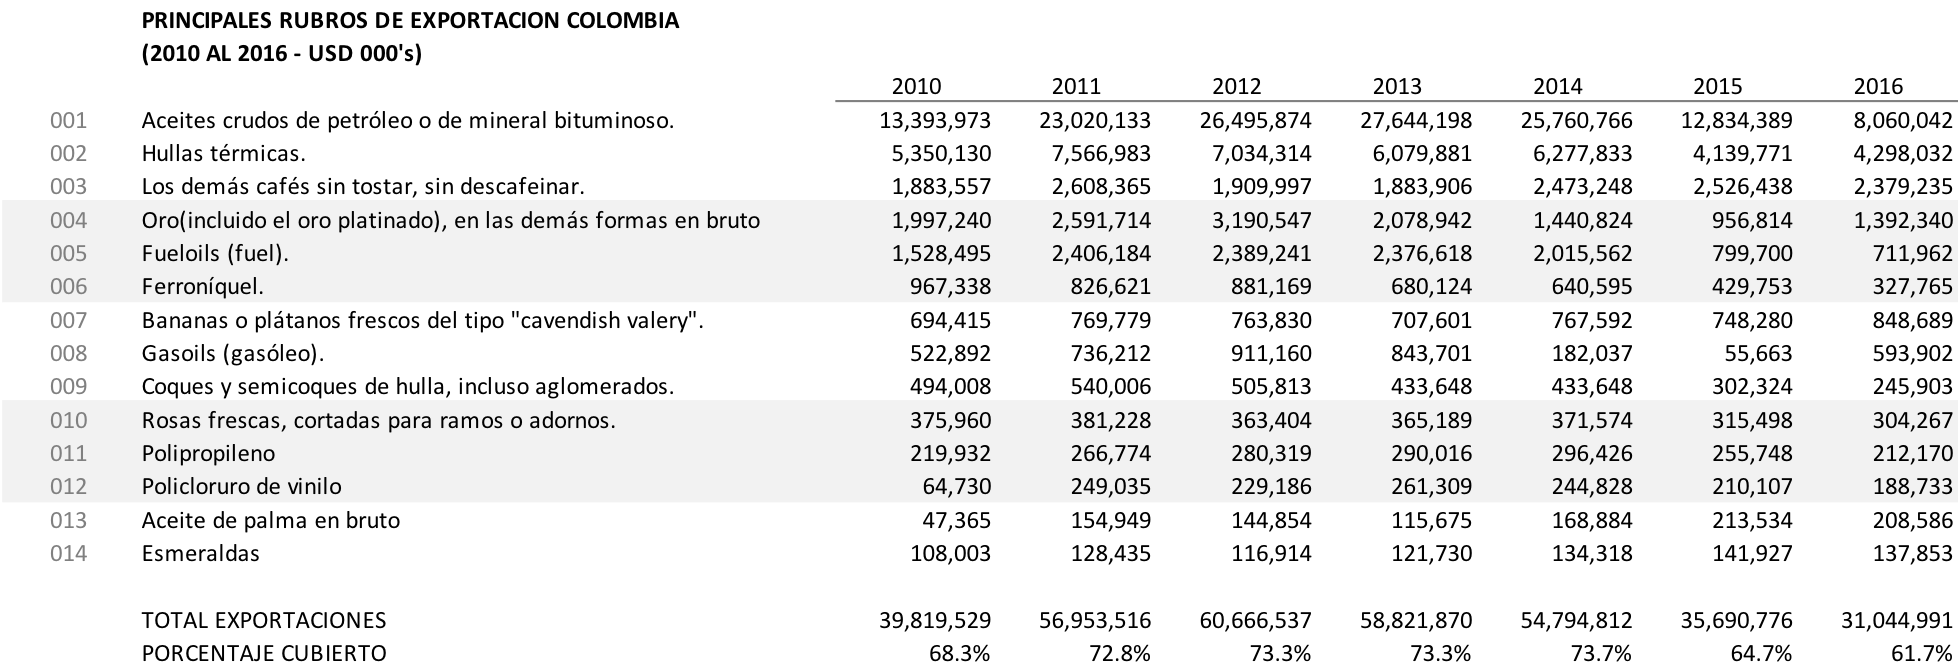
\includegraphics[width = 15cm]{ExportacionesColombia.png}
\caption{Principales Rubros de Exportación Colombia 2010-2016}
\end{figure}

\section{Regresión Lineal}
La regresión lineal es el punto de entrada más sencillo de entender y aplicar en la ciencia de datos. Parte de esto se debe a que la regresión lineal es aplicable en muchos casos a una gran gama de problemas de predicción en los cuales el científico de datos cuenta con una base de datos o juego de datos lo suficientemente grande y accesible para entrenar un modelo. La segunda razón es que un modelo bien entrenado de regresión lineal por lo general nos da una respuesta con cierto grado de precisión que da por cerrado el caso. 

El concepto en sí es relativamente sencillo de abstraer y explicar. En una visualización de datos donde un valor $y$ se corresponde con alguna relación del valor $x$, para cada $x$ y $y$, es posible trazar una línea que en cierta forma sea representativa del valor de predicción de $y$ para cada $x$. Esta línea puede no ser perfecta, o puede dejar muchos puntos sin una relación válida (a menos en el papel de gráfico) pero nos da una idea aproximada de la tendencia y evolución de los datos. \\

\begin{figure}[h!]
    \centering
    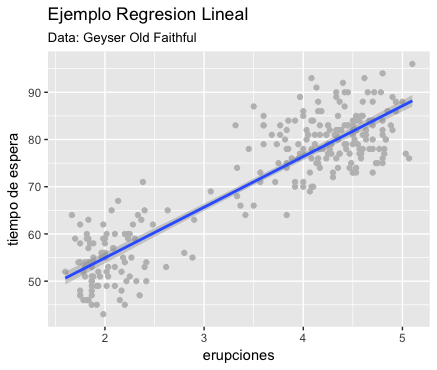
\includegraphics[width = 4 in]{ejemRegresionLineal.png}
    \caption{Ejemplo de Regresión Lineal con Old Geyser}
\end{figure}

Zumel y Mount describen la regresión lineal como el más común de los métodos de aprendizaje automatizado \cite{zumelMount}. Para los autores hay una probabilidad muy grande que el método funcione bien con el problema, y si no, es muy fácil verificar cual otro método probar como segunda opción. Para Daroczi, el énfasis está en los modelos de regresión multivariable (una extensión de la regresión lineal simple de un solo predictor y resultado) que construyen el camino para la predicción de fenómenos complejos en la naturaleza y negocios (Daróczi, G., 2015). Por su parte, Harrington resume los beneficios de la regresión lineal (Harrington, P., 2012) por la facilidad de interpretar los resultados y lo frugal en el uso de ciclos de computación (aunque puede ser menos útil si el fenómeno no es perfectamente lineal).

\subsection{Definición de Regresión Lineal}
Downey describe la regresión lineal como aquella que está basada en modelos de funciones lineales \cite{thinkStats}. Para Mann y Lacke la regresión lineal es aquella que se da como una función lineal entre dos variables, y la cual se puede dibujar en el plano cartesiano como una recta \cite{intoStats7}. Yau por su lado, define la regresión lineal simple como el modelo que describe la relación entre dos variables, $x$ y $y$, expresada por la ecuación de regresión lineal, donde $\alpha$ y $\beta$ son parámetros y $\epsilon$ es el término de error \cite{yau}.

La fórmula a la que hacemos referencia en la definición de Yau, y la que utilizan los otros autores, es la siguiente:

\[Y_{i} = \beta_{0} + \beta_{1}X_{i} + \epsilon_{i}\]

Dentro del aprendizaje automatizado la regresión tiene su propia interpretación donde se asume que el modelo está definido por un juego de parámetros \cite{alpaydin}:

\[ y = g(x \mid \theta) \]

donde $g(.)$ es el modelo y $\theta$ son sus parámetros. $Y$ es un número dentro de una regresión y $g(.)$ es la función de la regresión. El programa de aprendizaje automatizado optimiza los parámetros $\theta$ de forma que el error de aproximación sea mínimo, o en otras palabras, que los valores estimados sean los más cercanos a los valores reales del juego de entrenamiento. 

Los parámetros $\beta_{0}$ y $\beta_{1}$ determinan el punto en el que la función intercepta la la ordenada y la pendiente de la función. Podemos profundizar estos dos puntos aún más:
\begin{itemize}
	\item el punto de intercepción es la predicción del valor de $y$ cuando $x=0$. 
    \item la pendiente $\beta_{1}$ representa la predicción del aumento de $y$ con cada unidad que incrementa $x$
\end{itemize}

Notemos que las observaciones no están dispuestas en una línea recta, sino que se encuentran dispersas alrededor de esta. Debemos pensar de cada observación $\beta_{0} + \beta_{1}x_{i}$ como la parte sistemática del modelo, y $\epsilon_i$ como el error aleatorio. Este margen de error no es un error per se, pero una desviación del modelo lineal \cite{hyndman}. Asumimos que el factor de error cumple con los siguientes requisitos. 

\begin{enumerate}
  \item tiene media cero
  \item no contiene autocorrelación
  \item no está relacionado con la variable predictor
\end{enumerate}

Se espera que la distribución de los errores sea normal con varianza constante para producir pronósticos precisos. 

\subsection{Estimación con Mínimos Cuadrados}
En la práctica se tiene un juego de valores y no los mismos de $\beta_{0}$ y $\beta_{1}$. Estos necesitan ser calculados en base al juego de datos en lo que se conoce como el calce o ajuste de la linea a través de los datos. Hay muchas posibles líneas que calcen en el modelo con diferentes valores para $\beta_{0}$ y $\beta_{1}$. El método de mínimos cuadrados provee una forma de seleccionar valores para $\beta_{0}$ y $\beta_{1}$ minimizando la suma del error cuadrático:

\[ \sum_{i=1}^{N} \epsilon_{i}^{2} = \sum_{i=1}^{N}(y_{i} - \beta_{0} - \beta_{1}x_{i})^2 \]

Utilizando cálculo matemático, se ha demostrado que los estimados de los mínimos cuadrados son:

\begin{equation}
\begin{split}
	\hat{\beta}_{1} &= \frac{\sum_{i=1}{N}(y_{i}-\bar{y})(x_{i} - \bar{x})}{\sum_{i=1}{N}(x_{i}-\bar{x})^2}\\
	\hat{\beta}_{0} &= \bar{y} - \hat{\beta}_{1} \bar{x}\\
\end{split}
\end{equation}

\subsection{Regresión Multi-Variable}
Para Downey (Downey, 2015), la regresión múltiple es aquella en la cual se utilizan múltiples variables independientes, pero una sola variable dependiente. 

El Dr. Tattar de la Universidad de Bangalore define que el modelo de regresión línea simple no es realista ni aplicable al mundo practico (Tattar, 2013). Para aplicaciones más reales, es casi obligatorio el uso de modelos de regresión múltiple, en los cuales varias variables independientes se conjugan como parámetros de regresión. 

La regresión multivariable no es un tema mayormente complicado en teoría cómo lo es en llevar a la práctica. No todos los ejemplos de regresiones multivariables nos van a llevar a funciones lineales, sino que estamos tocando el limite entre regresión lineal y métodos de regresión general con funciones no lineales que pueden necesitar de transformaciones matemáticas para obtener un modelo apropiado \cite{daroczi}. Aquí también se explica la selección de un modelo con múltiples variables independientes y cuales conviene seleccionar \cite{viswanathan}.

La mayor parte de la teoría de esta sección sigue el desarrollo de la fórmula:

\[Y_{i} = \beta_{0} + \beta_{1}X_{1} + \beta_{2}X_{2} + \cdots + \epsilon_{i}\]

\subsection{Presunción del Modelo}
Hay cinco factores que deben darse en un modelo cuya presunción es que su muestra sigue una distribución normal. En esta sección revisamos cada uno de esos cinco factores \cite{daroczi}.

\subsubsection{Calce de los Datos}
Llegar a un modelo de regresión lineal no significa llegar a una solución optima, ni mucho menos. Los datos pueden calzar de forma muy elástica dentro del modelo, por lo que debemos recurrir a los coeficientes de correlación y determinación para verificar si el modelo tiene algún poder predictivo de uso científico

\subsubsection{R - Coeficiente de Correlación de Pearson}
El coeficiente de correlación de Pearson mide la relación lineal entre dos variables aleatorias cuantitativas. La correlación de Pearson es independiente de la escala de medida de las variables, lo que permite tener comparaciones mucho más objetivas independiente del fenómeno estudiado.

De manera menos formal, podemos definir el coeficiente de correlación de Pearson como un índice que puede utilizarse para medir el grado de relación de dos variables siempre y cuando ambas sean cuantitativas.

\[R = \frac{\Sigma(x_i - \bar{x})(y_i - \bar{y})}{\sqrt{\Sigma(x_i - \bar{x})^2\Sigma(y_i - \bar{y})^2}}\]

\subsubsection{R2 - Coeficiente de Determinación}
El coeficiente de determinación - denominado \(R^{2}\) - es un estadístico usado en el contexto de un modelo estadístico cuyo principal propósito es predecir resultados futuros o probar una hipótesis. El coeficiente determina la calidad del modelo para replicar los resultados, y la proporción de variación de los resultados que puede explicarse por el modelo. 

En el caso de regresión lineal, la formula del coeficiente de determinación sigue la siguiente forma:

\[R^{2} = \frac{\sigma^{2}_{XY}}{\sigma^{2}_{X}\sigma^{2}_{Y}}\]

\subsubsection{Valor de p}
\textbf{TEXTO INCOMPLETO - FALTA AGREGAR CONTENIDO}

\subsection{Seleccionando Variables de Predicción}
Un modelo de regresión de múltiple variables independientes puede tener una solución parsimoniosa sin necesidad de incluir todos sus términos. Esto es verdad cuando la cantidad de variables independientes utilizadas en el análisis 

\textbf{TEXTO INCOMPLETO - FALTA AGREGAR CONTENIDO}

\section{Series de Tiempo}
Muchos autores han escrito sobre las series de tiempo, pero es difícil agregar al tema o discutir las ideas del profesor Robert Hyndman, uno de los expertos más respetados en la comunidad de la estadística por su trabajo en las series de tiempo. Hyndman extiende la teoría a las series de tiempo como elementos de pronostico y su relación con la regresión lineal \cite{hyndman}. Desde el punto de vista técnico, Hyndman es el creador de varias bibliotecas de funciones de pronostico utilizando series de tiempo y ARIMA en lenguaje R. Dentro de la bibliografía, Daroczi es quien agrega detalles sobre la detección temprana de valores atípicos que pueden dificultar – y mucho – el análisis \cite{daroczi}. 

\subsection{Introducción a las Series de Tiempo}
Las series de datos son muy útiles para pronosticar algo que cambia con el tiempo. Ejemplos de estas cantidades que varían con el tiempo incluyen acciones en la bolsa de valor, cifras de ventas, y otro tipo de información cuantitativa \cite{hyndman}.

Una serie de tiempo es una serie de datos indexada en orden temporal. Comúnmente una serie de datos es una secuencia de datos tomados a puntos sucesivos y equidistantes en el tiempo, lo que la convierte en una secuencia de datos discretos en el tiempo. En forma general cualquier cosa que observamos secuencialmente en el tiempo es una serie de tiempos \cite{hyndman}. La literatura académica se concentra en series de tiempo que se observan en intervalos regulares de tiempo, aunque aquellas que se observan en intervalos irregulares también existen. 

El análisis de las series de tiempo es el uso de métodos para extraer estadísticas interesantes y otras características de los datos. El pronóstico de series de tiempo es el uso de modelos para predecir valores futuros basados en valores observados en el pasado. En el pronóstico de series de tiempo, la idea principal es estimar cómo la secuencia de observaciones continuará en el futuro. El pronóstico de series de tiempo utiliza solamente información de la variable a ser pronosticada, y no hace intento alguno de descubrir cuales son los factores que motivan este comportamiento (en análisis de regresión diríamos que buscamos las variables de confusión). Por lo tanto el análisis de series de tiempo extrapola la tendencia secular y los patrones cíclicas, pero ignora todo otro tipo de información que puede afectar el movimiento de la variable estudiada, como pueden ser en la vida real efectos de la publicidad en el lanzamiento de un producto, la tasa de cambio en las ventas, o actividades de riesgo en el precio internacional de materias primas. 

Podemos ver un ejemplo de serie de tiempo si tomamos los valores de la TRM (la Tasa Representativa de Mercado, el nombre oficial de la tasa de cambio del dólar en Colombia) en la siguiente gráfica:

\begin{figure}[h!]
    \centering
    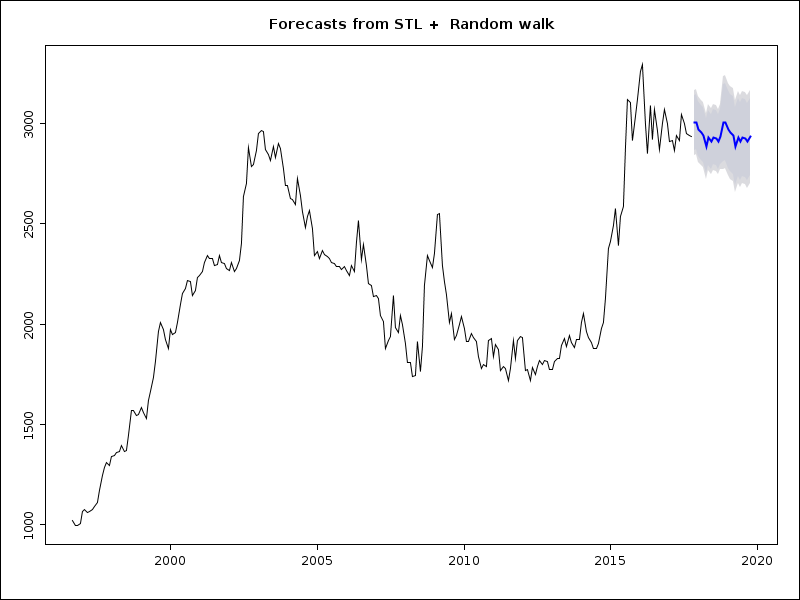
\includegraphics[width = 4 in]{timeSeries1.png}
    \caption{Ejemplo de Pronóstico con Descomposición STL (Fuente Hyndman and Athanasopoulos)}
\end{figure}

La línea negra es la variación de la TRM a lo largo del tiempo (en este caso, desde el año 1980 hasta el 2017). La línea azul es el pronóstico del valor de la TRM según la función \texttt{forecast()} del lenguaje R. La zona gris comprenden el intervalo de confianza del pronóstico, la cual nos da una idea más real de como puede fluctuar el pronóstico dentro del mismo.

La forma de una ecuación de series de tiempo se puede escribir en los siguientes términos:

\[ x(t+1) = f(x_t, x_{t-1}, x_{t-2}, \ldots, error) \]

Es posible utilizar predictores en el pronóstico de series de tiempo. Un ejemplo utilizando el tema de investigación de este mismo trabajo es el pronóstico de la TRM, la cual estimamos es el resultado de varios factores:

\[ TRM = f(\textnormal{demanda dólar, tasa interés, turismo, error}) \]

La relación no es exacta, sino que siempre habrá factores por lo cuales el modelo no puede responder. Estas variaciones están previstas en el término error dentro del modelo. Este tipo de modelo se llama \emph{modelo explanatorio}. 

Las series de tiempo se suelen catalogar en aditivas y multiplicativas. 

\begin{itemize}
	\item Las series aditivas son aquellas cuya variación en la estacionalidad, o variación en el ciclo o tendencia secular, no aumentan de forma proporcional al avance del tiempo.
	\item Las series multiplicativas son aquellas cuya variación en la estacionalidad, o variación en el ciclo o tendencia secular, aumentan de forma proporcional al avance del tiempo. Las series multiplicativas son comunes en ciencias como la economía y finanzas.
\end{itemize}

\subsection{Pronóstico con Series de Tiempo}
Los pronósticos con series de tiempo utilizan solamente la información disponible de la variable que se propone pronosticar, sin hacer intento alguno por descubrir los factores adicionales que condicionan su comportamiento. Por lo tanto se extrapolan las tendencias y patrones temporales, pero se ignora toda la información adicional como pueden ser iniciativas de publicidad, actividad de la competencia, cambios en las condiciones económicas y otros \cite{hyndman}.

\subsection{Patrones}
Las series de tiempo pueden descomponerse según su patrón o tendencia en tres elementos que las componen [Velazco, M., 2017]. A saber:

\begin{enumerate}
	\item Tendencia Secular: la tendencia secular o tendencia a largo plazo de una serie de tiempo es por lo común el resultado de factores a largo plazo. La tendencia no tiene porque ser lineal. Además es común ver que la tendencia cambia de dirección, ascendente o descendente \cite{hyndman}.
	\item Variación Estacional: Es el componente de la serie de tiempo que representa la variabilidad de los datos debido a la influencia de las estaciones. El componente de estacionalidad es siempre fijo \cite{hyndman}
	\item Variación Irregular: Esta variación se debe a factores a corto plazo, imprevisibles, y no recurrentes que afectan la serie de tiempo. Algunos autores llaman a estas variaciones \emph{cíclicas}. 
\end{enumerate}

Es importante saber distinguir entre los patrones cíclicos y estacionales. Los patrones estacionales tienen una duración fija y conocida en su extensión, mientras que los patrones cíclicos son mucho más extensos que los patrones estacionales y la duración de su magnitud es variable. La forma más sencilla es identificar los ciclos de estación con el calendario, por ejemplo los aumentos de tráfico en los centros comerciales en las fiestas de fin de año \cite{hyndman}. 

\subsection{Auto Correlación}
De igual manera que una correlación mide la extensión de una relación linear entre dos variables, la autocorrelación mide la relación linear entre dos valores retrasados de series de tiempo \cite{hyndman}.

El valor de una autocorrelación para un \(r_{k}\) dado es:

\[ r_{k} = \frac{\sum_{t = k + 1}^T(y_{t} - \bar{y})(y_{t - k} - \bar{y})}{\sum_{t = 1}^T(y_{t} - \bar{y})^{2}} \]

donde \(T\) es el valor de período temporal de la serie de tiempo. 

El autor Daroczi agrega como metodología para la verificación de autocorrelación en un juego de datos (no solo una serie de tiempos, sino cualquier juego de datos espacial) el \emph{Indice I de Moran} \cite{daroczi}. Dicho índice esta dado por la formula:

\[ I = \frac{N}{W} 
	\frac{\sum{i}\sum{j}w_{ij}(x_{i} - \bar{x})(x_{j} - \bar{x})}{{\sum{i}(x_{i} - \bar{x})^2}} \]

Los coeficientes de autocorrelación se visualizan a través de un gráfico de la función de autocorrelación o ACF (también llamado correlograma). Dicho gráfico analiza las relaciones entre valores retrasados de la serie de tiempo. Podemos utilizar la serie de tiempo representativa de la TRM para visualizar su gráfica de ACF.

\begin{figure}[h!]
    \centering
    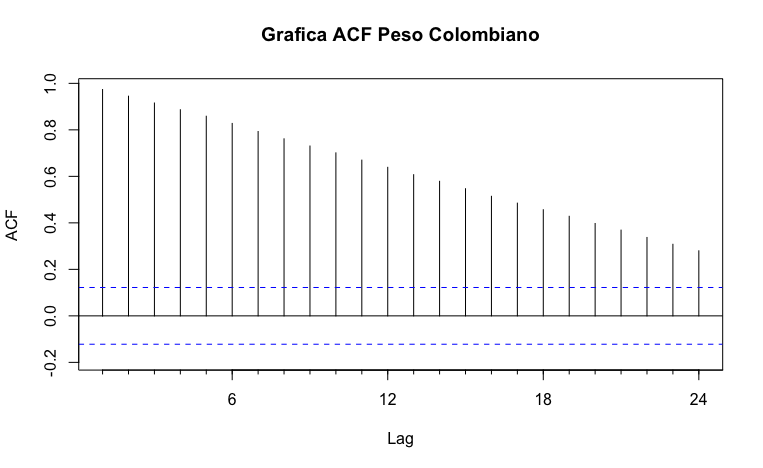
\includegraphics[width = 4 in]{COPEjemploACF.png}
    \caption{Correlograma del Peso Colombiano (Fuente propia)}
\end{figure}

Las series de tiempo que no muestran efectos de autocorrelación se denominan \emph{ruido blanco}. En dichas series se espera que los coeficientes de correlación sean cercanos a cero. Esto de por si es difícil, ya que toda serie de tiempo tendrá cierta variación aleatoria, pero en términos matemáticos esperamos que la serie tenga variaciones que 95\% del tiempo estén dentro de la región de $\pm2/\sqrt{T}$ donde $T$ es la extensión de la serie de tiempo. Si hay una o más series de magnitud fuera de estos límites, o si el 5\% o más de las series están fuera de estos límites, es muy probable que no sea ruido blanco \cite{hyndman}.

Existe una prueba adicional de autocorrelación que utiliza todo un grupo de datos $r_k$ en vez de tratarlos por separado. El racional para el proceso es que la visualización normal de una gráfica ACF es un test de hipótesis para cada retraso entre series. Cuando se hacen múltiples de estos test, la probabilidad de encontrar un falso positivo incrementa. Se evita este problema evaluando si las autocorrelación de los primeros $h$ valores es diferente de una serie de ruido blanco. El test de un grupo de valores con autocorrelación se conoce como un test \emph{portmanteau}. Uno de los más utilizados es el test \emph{Box-Pierce}:

\[ Q = T \sum_{k=1}^{h}r_{k\prime}^2 \]

donde $h$ es el retraso máximo considerado y $T$ es el número de observaciones. Si cada uno de los $r_k$ es cercano a cero, entonces Q sera mínimo. Si alguno de los valores de $r_k$ son grandes (ya sea positivos o negativos), entonces Q será grande. Hyndman y Athanasoupulos sugieren utilizar $h = 10$ para data no estacional y $h = 2m$ para datos con estacionalidad, donde $m$ es el número de estaciones, por ejemplo 4 para trimestres \cite{hyndman}.  El test \emph{Box-Pierce} tiende a no ser confiable con valores grandes de $h$. Si $h > T/5$ es recomendable utilizar $h=T/5$.

Un test relacionado - y más preciso - es el test \emph{Ljung-Box}:

\[ Q* = T(T+2) \sum_{k=1}^{h}(T-k)^{-1}r_{k\prime}^{2} \]

Si el valor de $Q*$ es grande, las autocorrelaciones no provienen de una serie de ruido blanco. 

\subsection{Precisión del Pronóstico}
Para el estudio de la precisión del pronóstico de series de tiempo, sea $y_i$ la observación $i$ de datos y $\hat{y_i}$ el pronóstico de $y_i$.

\subsubsection{Errores dependiente de la Escala}
El error del pronóstico es la diferencia $e_i = y_i - \hat{y_i}$, que está en la misma escala que los datos. Las medidas de precisión que dependen de $e_i$ son dependientes de la escala y no se pueden utilizar para hacer comparaciones entre series de tiempo de diferentes escalas. Las dos formas que se utilizan comúnmente para medir la precisión del pronóstico de series de tiempo dependiente de escalas están basadas en el error absoluto o error cuadrático \cite{hyndman}. Se trata de:

\begin{eqnarray*}
	\text{Error Promedio Absoluto (MAE)}& = &\text{promedio}(|e_{i}|) \\
	\text{Error Promedio Cuadrático (RMSE)}& = &\sqrt{promedio_{e_1}^2} 
\end{eqnarray*}

La tendencia al comparar precisión en un solo juego de datos es utilizar el MAE ya que es mas sencillo y simple de entender. 

\subsubsection{Errores Porcentuales}
Un error porcentual es del tipo $p_i = 100 e_i / y_i$. Los errores porcentuales son independientes de la escala, y se utilizan con facilidad para comparar errores en la precisión de múltiples juegos de datos. Es error porcentual más común es:

\[ \text{Error Promedio Porcentual Absoluto (MAPE)} = promedio(\mid p_i \mid) \]

Las medidas basadas en errores porcentuales tienen la debilidad de ser infinitas o indefinidas cuando $y_i = 0$ para cualquier $i$. Esto también ocurre cuando un $y_i$ tiende a cero. 

\subsection{Descomposición de Series de Tiempo}
La descomposición de las series de tiempo facilita el análisis y la investigación exploratoria de los datos. Una de las formas mas sencillas de lograr esto es la aplicación de promedios móviles, lo cual se facilita mucho en R con el uso de la función \texttt{decompose()} \cite{daroczi}.

Pensemos en la serie de tiempo $y_t$ compuesta por tres factores: un componente estacional, un componente de tendencia (que contiene tanto tendencia secular como cíclica) y un último componente que contiene cualquier otro resto de información importante. Podemos entonces escribir una serie de tiempos aditiva como:

\[ y_t = S_t + T_t + E_t \]

donde $y_t$ es la data en el período $t$, $S_t$ es el componente estacional en el período $t$, $T_t$ es el componente de tendencia-ciclo en el período $t$, y $E_t$ es el componente de error en el período $t$. De forma alternativa podemos escribir una ecuación similar para los modelos de series de datos multiplicativos como:

\[ y_t = S_t * T_t * E_t  \]

El modelo aditivo es más apropiado si la magnitud de las fluctuaciones estacionales o la variación alrededor del ciclo o tendencia no varía con los niveles de la serie de tiempo (ejemplo: el avance del tiempo). Cuando la variación se da, o sea es proporcional con el avance del tiempo en la serie, un modelo multiplicativo es más apropiado. Este es el caso de la mayoría de las series de tiempo en la economía \cite{hyndman}.

\subsubsection{Datos Ajustados Estacionalmente}
Si el componente de estacionalidad se elimina de la serie de datos original, los valores resultantes se denominan \emph{ajustados estacionalmente}. Para un modelo aditivo, el ajuste por estacionalidad se da por $y_t - S_t$. Para un modelo multiplicativo este se da por $y_t/S_t$. Si la variación por estacionalidad no es de importancia, la serie ajustada por estacionalidad puede ser útil. Estos casos se dan por ejemplo con los datos de desempleo mensual, los cuales se saben tienen variación estacional que altera la lectura real del cambio. 

\subsubsection{Métodos de Descomposición de Series de Tiempo}
Existen múltiples métodos de descomposición de series de tiempo. En nuestro marco teórico tocaremos brevemente los de promedios móviles, promedios móviles ponderados, STL, suavizar exponencialmente, y ARIMA.

\subsubsection{Promedios Móviles}

El método de promedios móviles origina de los años 1920 y fue ampliamente utilizado hasta los 1950. Hasta el día de hoy es la base de todos los otros métodos modernos de descomposición. El fundamento del mismo es utilizar los promedios móviles para estimar la tendencia o ciclo \cite{hyndman}. La descomposición por promedios móviles toma la forma siguiente:

\[ \hat{T}_{t} = \frac{1}{m} \sum_{j = -k}^{k} y_{t + j}  \]

donde $m=2k+1$. Esto significa que el estimado de la tendencia/ciclo en el momento $t$ se obtiene promediando los valores de la serie de tiempo dentro de $k$ períodos de $t$ valores. 

\subsubsection{Promedios Móviles Ponderados}
Es posible obtener promedios móviles de los promedios móviles. Combinaciones de estos nos dan promedios ponderados. Por ejemplo un modelo 2X4-MA, que es un promedio de promedios móviles, es el equivalente a un modelo 5-MA con ponderaciones dadas por el vector de pesos $[\frac{1}{8}, \frac{1}{4}, \frac{1}{4}, \frac{1}{4}, \frac{1}{8}]$ \cite{hyndman}. La forma de escribir un modelo de promedios móviles ponderados es la siguiente:

\[ \hat{T}_{t} = \sum_{j = -k}^{k} a_j y_{t + j}  \]

donde $k=(m-1)/2$ y los pesos están dados por $[a_{-k}, \ldots, a_{k}]$. Es importante que todos los pesos sumen uno como valor y que sean simétricos para que $a_{j} = a_{-j}$. Una ventaja mayor de los promedios móviles ponderados es que producen estimados más suavizados de la tendencia/ciclo. 

\subsubsection{Descomposición STL}
El método STL es muy versátil y robusto para la descomposición de series de tiempo. Su nombre es el acrónimo en inglés de \emph{Seasonal and Trend Descomposition using Loess}, que significa descomposición de estacionalidad y tendencia utilizando Loess. Loess es un método para estimar relaciones no-lineales desarrollado por Cleveland et al \cite{hyndman}. Las desventajas de STL es su manejo de cierta data financiera (como por ejemplo días de comercio bursátil) y las variaciones de calendario. La biblioteca de R tiene una función que descompone automáticamente una serie de datos utilizando STL, la función \texttt{STL()}.

La descomposición STL se utiliza más que nada para estudiar las series de tiempo, pero tiene aplicación en pronosticar. Asumiendo una descomposición aditiva, la serie de tiempo descompuesta se puede escribir como:

\[ y_{t} = \hat{S}_t + \hat{A}_t \]

donde $\hat{A}_t = \hat{T}_t + \hat{E}_t$ es el componente ajustado por estacionalidad. Si se trata de una serie multiplicativa entonces la misma ecuación se puede escribir como: 

\[ y_{t} = \hat{S_t}\hat{A_t}\]

donde $\hat{A}_t = \hat{T}_t\hat{E}_t$. 

Para pronosticar cualquier componente ajustado por estacionalidad, se puede utilizar cualquier método de pronóstico no estacional. Por ejemplo, se puede aplicar camino aleatorio con deriva, Holts-Winter, o ARIMA.

\subsubsection{Alisamiento Exponencial}
El Alisamiento Exponencial (o Suavizamiento Exponencial según la traducción), fue propuesto por Brown, Holt y Winters entre los años 1950 a 1960. Los pronósticos producto del suavizamiento exponencial son promedios ponderados de observaciones históricas en las cuales el valor del peso va decayendo a medidas que las observaciones van envejeciendo. En otras palabras, las observaciones más nuevas reciben mayor asociación con el peso. 

La primera forma de suavizamiento exponencial se llama \emph{suavizamiento exponencial simple}. Este método es aplicable para el pronóstico de series de datos sin tendencia o estacionalidad. El pronostico se calcula con promedios ponderados donde los pesos decrecen exponencialmente a medida que las observaciones envejecen - los pesos más pequeños se asocian con las observaciones más antiguas. 

\[ \hat{y}_{T+1 \mid T} = \alpha y_{T} + \alpha(1-\alpha) y_{T-1} + \alpha(1-\alpha)^2 y_{T-2} + \alpha(1-\alpha)^3 y_{T-3} + \ldots \]

donde $0 \leq \alpha \leq 1$ es el parámetro de alisamiento. El pronóstico de $T + 1$ es el promedio ponderado de todas las observaciones en la serie $y_1, \ldots, y_T$. La tasa por la cual decrecen los pesos se controla con el parámetro $\alpha$.

Este método se puede extender aplicando el factor de suavizamiento exponencial decreciente para lograr la ecuación de la segunda forma de suavizamiento exponencial ponderado de tal forma que:

\[ \hat{T}_{T+1 \mid T} = \sum{j=0}^{T-1} \alpha(1-\alpha)^j y_{T-j} + (1-\alpha)^{T} \ell_{0}  \]

Notemos que la ecuación es otra forma de escribir la notación del suavizamiento exponencial simple. 

Holt extendió el método de suavizamiento exponencial para permitir hacer pronósticos con datos que contenían tendencia \cite{hyndman}. Este método de pronóstico incluye una ecuación de pronóstico y dos ecuaciones de suavizamiento, una para el nivel y otra para la tendencia:

\begin{eqnarray*}
	\text{Ecuación de Pronóstico}&&\hat{y}_{t+h \mid t} = \ell_{t} + hb_{t} \\
	\text{Ecuación de Nivel}&&\ell_{t} = \alpha y_{t} + (1 - \alpha)(\ell_{t-1} + b_{t-1}) \\
	\text{Ecuación de Tendencia}&&b_{t} = \beta^{*}(\ell_{t} - \ell_{t-1}) + (1 - \beta^{*})b_{t-1}  
\end{eqnarray*}

donde $\ell_{t}$ denota el nivel estimado de la serie de tiempo en el momento $t$, $b_{t}$ denota el estimado de la tendencia de la serie de tiempo en el momento $t$, $\alpha$ es el parámetro de suavizamiento para el nivel, $0 \lq \alpha \leq 1$ y $\beta^{*}$ es el parámetro de suavizamiento de la tendencia, $0 \leq \beta^{*} \leq 1$.

Holt y Winters volverían sobre el método de Holt para extenderlo y capturar el elemento de estacionalidad, el único que faltaba en la ecuación. El método \emph{Holt-Winters} está compuesto por una ecuación de pronóstico y tres de suavizamiento - una para el nivel $\ell_{t}$, una para la tendencia $b_{t}$, y otra para el componente estacional $S_t$, con los parámetros de suavizamiento $\alpha$, $\beta^{2}$, y $\gamma$. Se utiliza $m$ para definir el período de estacionalidad, por ejemplo el número de temporadas en el año. De tal forma los meses serían $m=12$. 

Hay dos variaciones del método que difieren en la naturaleza de los componentes de estacionalidad. El método aditivo es preferible cuando las variaciones de estacionalidad son más o menos constantes a través de la serie. El método multiplicativo es preferible cuando la variación de estacionalidad son cambiantes proporcionalmente al nivel de las series. 

Los componentes de la forma aditiva son los siguientes:

\begin{equation} 
\begin{split}
	\hat{y}_{t+h \mid t} & = \ell_{t} + hb_{t} + s_{t-m+h_{m}^{+}} \\
 	\ell_{t} & = \alpha(y_{t} - s_{t-m}) + (1 - \alpha)(\ell_{t-1} + b_{t-1}) \\
    b_{t} & = \beta^{*}(\ell_{t} - \ell_{t-1}) + (1 - \beta^{*})b_{t-1} \\
    s_{t} & = \gamma(y_{t} - \ell_{t-1} - b_{t-1}) + (1-\gamma)s_{t-m}
\end{split}
\end{equation}

donde $h_{m}^{+} = \lfloor (h-1) mod m \rfloor + 1$, son los que regulan que el estimado de los índices estacionales usados para el pronóstico vengan del año final de la serie. La ecuación de nivel nuestra el promedio ponderado entre la observación ajustada por estacionalidad $(y_{t} - s_{t-m}$ y el pronóstico no ajustado $(\ell_{t-1} + b_{t-1})$ para el momento $t$. La ecuación de la tendencia es idéntica al método lineal de Holt. La ecuación de la estacionalidad muestra un promedio ponderado el índice estacional actual, $(y_{t} - \ell_{t-1} - b_{t-1})$, y el índice para la misma temporada en el período previo (por ejemplo, $m$ períodos atrás).

Los parámetros de la ecuación $\ell_{t}$, $b_{t}$ y $s_{t}$ se corrigen por error dentro de la ecuación de suavizamiento con las siguientes fórmulas:

\begin{equation}
\begin{split}
	\ell_{t} & = \ell_{t-1} + b_{t-1} + \alpha e_{t} \\
    b_{t} & = b_{t-1} + \alpha \beta^{*} e_{t} \\
    s_{t} & = s_{t-m} + \gamma e_{t} \\
\end{split}
\end{equation}

Los componentes del método \emph{Holt-Winters} para modelos multiplicativos son los siguientes:

\begin{equation} 
\begin{split}
	\hat{y}_{t+h \mid t} & = (\ell_{t} + hb_{t}) s_{t-m+h_{m}^{+}} \\
 	\ell_{t} & = \alpha \frac{y_{t}}{s_{t-m}} + (1 - \alpha)(\ell_{t-1} + b_{t-1}) \\
    b_{t} & = \beta^{*}(\ell_{t} - \ell_{t-1}) + (1 - \beta^{*})b_{t-1} \\
    s_{t} & = \gamma \frac{y_{t}}{(\ell_{t-1} - b_{t-1})} + (1-\gamma)s_{t-m}
\end{split}
\end{equation}

Las ecuaciones para la corrección de errores son las siguientes:

\begin{equation}
\begin{split}
	\ell_{t} & = \ell_{t-1} + b_{t-1} + \alpha \frac{e_{t}}{s_{t-m}} \\
    b_{t} & = b_{t-1} + \alpha \beta^{*} frac{e_{t}}{s_{t-m}} \\
    s_{t} & = s_{t} + \gamma frac{e_{t}}{(\ell_{t-1} + b_{t-1})} \\
\end{split}
\end{equation}

donde $e_{t} = y_{t} - (\ell_{t-1} + b_{t-1})s_{t-m}$.

\subsection{ARIMA}
Los modelos ARIMA son otro enfoque para el pronóstico de series de tiempo. Mientras que la metodología de suavizamiento exponencial busca la descripción de la tendencia y estacionalidad de la data, los modelos ARIMA intentan describir la autocorrelación de la misma. 

\subsubsection{Series de Tiempo Estacionarias}
Un requisito para el modelar pronósticos con series de tiempo es que las mismas deben ser estacionarias \cite{srivastava}. Por lo tanto es importante definir la estacionalidad de series de tiempo antes de avanzar con la descomposición de las mismas. 

Definimos una serie de tiempo estacionaria como aquella cuyas propiedades no dependen del momento en la cual se la observa \cite{hyndman}. Por lo tanto las series de tiempo con tendencias, o con estacionalidad, no son estacionarias. La tendencia o la estacionalidad afectará el valor de la serie de tiempos en momentos específicos de la misma. Una serie de ruido blanco es un caso de series de tiempo estacionarias. En casos puede ser confuso determinar que es que. Una serie de tiempos puede ser cíclica y estacionaria si cumple con la condición de no tener tendencia o estacionalidad.

Hay tres criterios básicos que debe cumplir una serie de tiempos para catalogarla como estacionaria \cite{srivastava}:

\begin{enumerate}
	\item El promedio de la serie no debiera ser una función del tiempo sino una constante. Esto es visible a la vista en una serie de tiempos que permanece relativamente horizontal sobre el eje de la abscisa a pesar de fluctuar. 
	\item La varianza de la serie no debiera ser una función del tiempo. Esta propiedad se conoce en matemática como \emph{homocedasticidad}.
    \item La covarianza del término $x_i$ y el término $(x + m)_i$ no debiera ser una función en el tiempo. Esto también posible de ver en una gráfica, a medida que la función disminuye la distancia entre sus ondas, o aumenta la densidad de las mismas proporcional avanza en el tiempo. 
\end{enumerate}

El académico Tavish Srivastava agrega sobre el concepto de series estacionarias la necesidad de asociar el de \emph{random walk} o camino aleatorio. Una serie de tiempo es un camino aleatorio con promedio cero pero con varianza dependiente en el tiempo, por lo tanto no es una serie estacionaria \cite{srivastava}.

\subsubsection{Diferenciando Series de Tiempo}
Una forma de convertir una serie de tiempo en estacionaria es diferenciarla. Al diferenciarla, se toma las diferencias entre observaciones consecutivas de la serie. La diferenciación ayuda a estabilizar el promedio de una serie de tiempos removiendo cambios en el nivel de la misma y eliminando - o por lo menos reduciendo - se tendencia y estacionalidad \cite{hyndman}. 

Para una serie de tiempos estacionaria, su ACF disminuirá a cero relativamente rápido, mientras que el cuadro ACF de una serie no estacionaria disminuirá de forma paulatina y lenta. Además, para una serie no estacionaria, su valor $r_1$ es por lo general grande y positivo \cite{hyndman}.

\begin{figure}[h!]
    \centering
    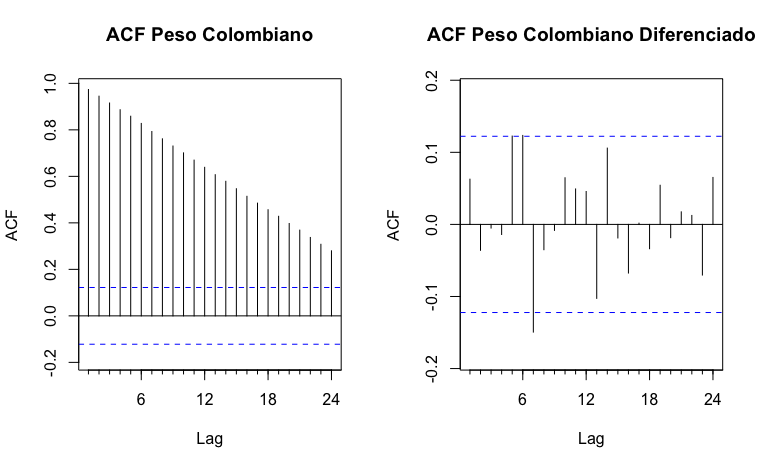
\includegraphics[width = 4 in]{DiffEjemploACF.png}
    \caption{Correlograma del Peso Colombiano Con y Sin Diferenciar (Fuente propia)}
\end{figure}

Una serie diferenciada es el cambio entre dos observaciones consecutivas y puede detallarse de la siguiente forma:

\[ y_{t}^{\prime} = y_{t} - y_{t-1} \]

Una serie diferenciada tendrá solo $T-1$ valores dado que no es posible calcular la diferencia $y_{1}^{\prime}$ para la primera observación. Cuando la serie diferenciada es ruido blanco, se la puede definir como:

\[ y_{t} = y_{t-1} - e_{t} \]

Las diferenciaciones también pueden hacerse por temporadas. Una diferenciación estacional es la diferencia entre una observación y su observación correspondiente del período pasado:

\[ y_{t}^{\prime} = y_{t} - y_{t-m} \]

donde $m$ es igual al número de temporadas. Estas se conocen como \emph{diferencias de m-retrasos}.

\subsubsection{Pruebas de Raíz Unitaria}
Una forma de determinar más objetivamente si hay necesidad de diferenciar una serie es la \emph{prueba de raíz unitaria}. Estas son pruebas de hipótesis estadísticas que están diseñadas para determinar la necesidad o no de diferenciación de la serie \cite{hyndman}. Existen varias y están basadas en diferentes enfoques, por lo que es común utilizar más de una si hay respuestas conflictivas que confrontar. 

La más utilizada es la prueba aumentada \emph{Dickey-Fuller}, también conocida como \emph{ADF}. Para este test, se utiliza el siguiente modelo de regresión \cite{dickeyfuller}:

\[ y_{t}^{\prime} = \phi y_{t-1} + \beta y_{t-1}^{\prime} + \beta_{2} y_{t-2}^{\prime} + \ldots + \beta_{k} y_{t-k}^{\prime} \]

donde $y_{t}^{\prime}$ denota la primera serie diferenciada, $y_{t}^{\prime} = y_{t} - y_{t-1}$ y $k$ es el número de retrasos para incluir en la regresión (que por regla común se ajusta a 3). Si la serie original, $y_{t}$, necesita diferenciarse, entonces el coeficiente $\hat{\phi}$ debiera aproximar a cero. Si $y_{t}$ ya es estacionaria, $\hat{\phi} < 0$. La metodología normal de test de hipótesis no funciona cuando la serie es estacionaria, pero el lenguaje \emph{R} tiene una función que lo calcula sin problemas de la forma \texttt{adf.test(x, alternative="stationary")} \cite{packageForecast}.

La hipótesis nula para una prueba \emph{Dickey-Fuller} es que la data es no-estacionaria. De tal manera que valores grandes de $p$ son indicativos de no-estacionalidad y valores pequeños de $p$ por el contrario indican que la hipótesis alternativa es de serie estacionaria. Un corolario de esto es que se necesita usar diferenciación cuando $p > 0.05$. 

\subsubsection{Modelos Autoregresivos (AR)}
En un modelo de regresión múltiple, pronosticamos la variable de interés usando una combinación lineal de predictores. En un modelo autoregresivo, el pronóstico de la variable de interés se conforma con una combinación lineal de valores pasados de la variable. El término autoregresión indica que es una regresión de variables contra si mismas \cite{hyndman}. 

Por lo tanto un modelo autogresivo de orden $p$ puede ser escrito como:

\[ y_{t} = c + \phi_{1}y_{t-1} + \phi_{2}y_{t-2} + \ldots + \phi_{p}y_{t-p} + e_{t}  \]

donde $e_{t}$ es ruido blanco. Es muy similar a la regresión múltiple pero con valores retrasados de $y_{t}$ como predictores. Esto se refiere a un modelo \textbf{AR(p)}. Los modelos autoregresivos son muy flexibles para manejar un portafolio amplio de patrones de series de datos. El cambio de los parámetros $\phi_1, \ldots, \phi_{p}$ resulta en diferentes patrones de series de datos. La varianza del término de error $e_t$ solo modifica la escala de la serie, no los patrones.

\subsubsection{Modelos de Promedios Móviles (MA)}
En vez de utilizar los valores pasados de una variable de pronóstico en una regresión, el modelo de promedios móviles utiliza los errores pasados del pronóstico en un modelo cuasi-regresión.

\[ y_{t} = c + e_{t} + \phi_{1}e_{t-1} + \phi_{2}e_{t-2} + \ldots + \phi_{q}e_{t-q} \]

donde $e_{t}$ es ruido blanco. Nos referimos a este modelo como \textbf{MA(q)}. En realidad no observamos los valores de $e_{t}$, por lo que no es una regresión en el sentido estricto de la palabra \cite{hyndman}. Hacemos notar que cada valor de $y_{t}$ puede ser pensado como un promedio móvil ponderado de los últimos errores de pronóstico. Sin embargo no hay que confundirlo con el suavizamiento de promedios móviles. El cambio de los parámetros $\phi_1, \ldots, \phi_{p}$ resulta en diferentes patrones de series de datos. Al igual que en los modelos autoregresivos, la variación del término de error $e_t$ solo modifica la escala de la serie, no los patrones.

\subsubsection{Modelos ARIMA No-Estacionarios}
Si combinamos la diferenciación con la autoregresión y un modelo de promedios móviles, obtenemos el \emph{modelo no-estacionario ARIMA}. ARIMA es el acrónimo para \emph{AutoRegressive Integrated Moving Average} (o modelos autoregresivos integrados de promedios móviles). En este caso son integrados porque la integración es la función opuesta de diferenciación \cite{hyndman}. Podemos escribir el modelo completo como:

\[ y_{t}^{\prime} = c + \phi_{1}y_{t-1}^{\prime} + \ldots + \phi_{p}y_{t-p}^{\prime} + \phi_{1}e_{t-1} + \ldots + \phi_{q}e_{t-q} + e_{t} \]

donde $y_{t}^{\prime}$ es la serie diferenciada (puede haber sido diferenciada más de una vez). Los predictores en la mano derecha de la ecuación incluyen tanto valores rezagados de $y_t$ y errores rezagados. A esto lo llamamos un modelo \textbf{ARIMA(p, d, q)}, donde:

\begin{description}
  \item [p = ]
  orden de la parte autoregresiva;
  \item [d = ]
  grado de la primera diferenciación involucrada; 
  \item [q = ]
  orden de la parte de promedios móviles.
\end{description}

Las mismas condiciones de estacionalidad e invertibilidad que se utiliza en los modelos de autoregresión y promedios móviles aplican al modelo ARIMA. 

\subsubsection{Gráficas ACF y PACF}
Seleccionar el juego indicado de variables \emph{p, d, q} puede ser difícil. Las bibliotecas de \emph{R} tienen funciones para ayudar. Por lo general no es posible a simple vista evaluar estos valores. Sin embargo, si es posible utilizar las gráficas de la función de autocorrelación ACF y su función asociada PACF para seleccionar valores de \textit{p} y \textit{q}. La gráfica de la función PACF mide la autocorrelación parcial entre $y_{t}$ y $y_{t-k}$ después de eliminar los efectos de otras series rezagadas $1, 2, 3, \ldots, k-1$. Por lo tanto la primer autocorrelación parcial es idéntica a la primer autocorrelación, porque no hay nada que eliminar. 

\begin{figure}[h!]
    \centering
    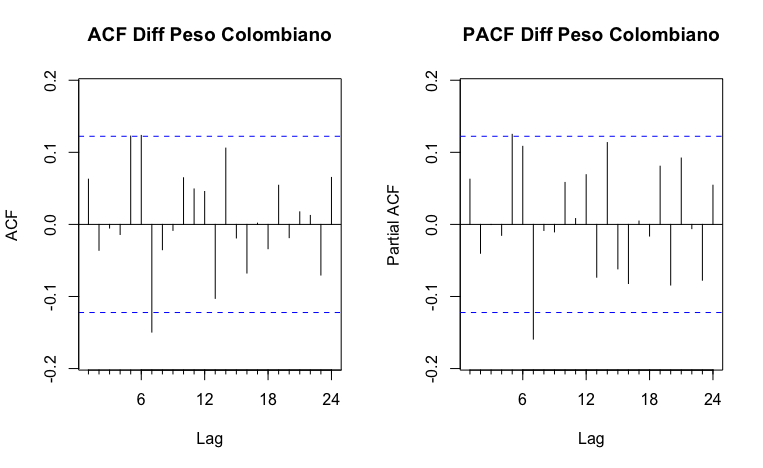
\includegraphics[width = 4 in]{ACFPACFEjemplo.png}
    \caption{Gráficas de las Funciones ACF y PACF del Peso Colombiano (Fuente propia)}
\end{figure}

Si los datos son de un modelo \textit{ARIMA(p,d,0)} o \textit{ARIMA (0,d,q)}, entonces las gráficas ACF y PACF pueden ser útiles en determinar los valores de \emph{p} o \emph{q}. Si tanto \emph{p} y \emph{q} son positivas, los gráficos no podrán ayudar a determinar los valores adecuados de \emph{p} y \emph{q}. 

Los datos pueden seguir un modelo ARIMA(p,d,0) si el gráfico ACF y PACF de los datos diferenciados muestran los siguientes patrones. 
\begin{itemize}
	\item la gráfica ACF decrece exponencialmente o tiene forma sinusoide 
	\item hay un crecimiento significativo en el tramo \textit{p} en la gráfica PACF, pero ninguno después del tramo \textit{p}
\end{itemize}

Los datos pueden seguir un modelo ARIMA(0,d,q) si el gráfico ACF y PACF de los datos diferenciados muestran los siguientes patrones. 
\begin{itemize}
	\item la gráfica PACF decrece exponencialmente o tiene forma sinusoide 
	\item hay un crecimiento significativo en el tramo \textit{p} en la gráfica ACF, pero ninguno después del tramo \textit{p}
\end{itemize}

\section{La Ciencia de Datos}
La Ciencia de Datos es una disciplina relativamente nueva, inclusive en muchos entornos académicos. El objetivo de este capítulo es el de resumir los aspectos mayores de la ciencia de datos como estudio multidisciplinario cuya intención es hacer sentido de la gran cantidad de datos que surgen de nuestro entorno, con miras a modificar los fenómenos del mundo.

\subsection{Introducción}
La ciencia de datos \cite{zumelMount} utiliza herramientas de otras ciencias empíricas, estadística, análisis matemático, finanzas, técnicas de visualización, inteligencia de negocios, sistemas expertos, aprendizaje automatizado, bases de datos, bioestadística, y ciencia de la computación con la finalidad de procesar y extraer conocimiento de la data, ya sea que esta se encuentre estructurada o no estructurada. 

Previo al termino Ciencia de Datos, el matemático John W. Tukey comienza a circular la idea del análisis de datos versus la estadística en su libro \textit{The Future of Data Analysis} \cite{tukey}. La premisa es que la estadística es una ciencia formal, mientras que el análisis de datos es una ciencia empírica ya que se basa en datos extraídos de la vida real. Tukey sostuvo que de la data debía extraerse hipótesis para evaluación, y que el análisis confirmatorio de datos debía coexistir al lado del análisis exploratorio de datos. Ambos se apoyan en la estadística como disciplina de aplicación pero estudian objetos diferentes. 

La ciencia de datos \cite{wikipediaDS} ha resultado para muchos una disciplina de reciente creación, pero en la realidad este concepto lo utilizó por primera vez el científico danés Peter Naur en la década de los sesenta como sustituto de las ciencias computacionales. En 1974 publicó el libro Concise Survey of Computer Methods 3 donde utiliza ampliamente el concepto ciencia de datos, lo que permitió que se comenzara a utilizar más libremente entre el mundo académico \cite{naur}.  

Por otro lado, el matemático japones e inventor de la \textit{Metodología de Cuantificación} Chikio Hayashi define sucintamente \cite{hayashi} la ciencia de datos no solo como un concepto sintético para unificar las disciplinas de la estadística, el análisis de datos, y sus métodos relacionados, sino por la forma en la cual sus resultados se aplican. Esta nueva metodología incluye tres fases: diseño de la data, recolección de la data, y análisis de la misma. 

Muchas veces se ha criticado a la ciencia de datos como el uso disimulado de estadística bajo un nombre diferente con fines comerciales. En 2001, William S. Cleveland introdujo a la ciencia de datos como una disciplina independiente, extendiendo el campo de la estadística para incluir los avances en computación con datos en su artículo \textit{Ciencia de datos: un plan de acción para expandir las áreas técnicas del campo de la estadística}. Cleveland estableció seis áreas técnicas que en su opinión conformarían al campo de la ciencia de datos: investigaciones multidisciplinarias, modelos y métodos para datos, computación con datos, pedagogía, evaluación de herramientas, y teoría \cite{cleveland}.

En abril del 2002, el \textit{ Council for Science: Committee on Data for Science and Technology} \cite{CODATA} empezó la publicación del \textit{Data Science Journal}, enfocada en problemas como la descripción de sistemas de datos, su publicación en Internet, sus aplicaciones y problemas legales. Poco después, en enero del 2003, la Universidad de Columbia empezó a publicar \textit{The Journal of Data Science}, la cual ofreció una plataforma para que todos los profesionales de datos presentaran sus perspectivas e intercambiaran ideas \cite{wikipediaDS}.

\subsection{El Científico de Datos y su Rol como Investigador}
Las personas que se dedican a la ciencia de datos se les conoce como científico de datos. El proyecto \textit{Master in Data Science} define al científico de datos como una mezcla de estadísticos, computólogos y pensadores creativos, con las siguientes habilidades:

\begin{itemize}
	\item Recopilar, procesar y extraer valor de las diversas y extensas bases de datos.
	\item Imaginación para comprender, visualizar y comunicar sus conclusiones a los no científicos de datos.
	\item Capacidad para crear soluciones basadas en datos que aumentan los beneficios, reducen los costos.
\end{itemize}

Los científicos de datos trabajan en todas las industrias y hacen frente a los grandes proyectos de datos en todos los niveles. La definición mas famosa de las habilidades que componen a un científico de datos se han atribuido al Dr. Nathan Yau \cite{yau}, quien precisó lo siguiente: \begin{quote} el científico de datos es un estadístico que debería aprender interfaces de programación de aplicaciones (API), bases de datos y extracción de datos; es un diseñador que deberá aprender a programar; y es un computólogo que deberá saber analizar y encontrar datos con significado. \end{quote}

En la tesis doctoral de Benjamin Fry \cite{fry} explicó que el proceso para comprender mejor a los datos comenzaba con una serie de números y el objetivo de responder preguntas sobre los datos, en cada fase del proceso que él propone (adquirir, analizar, filtrar, extraer, representar, refinar e interactuar), se requiere de diferentes enfoques especializados que aporten a una mejor comprensión de los datos. Entre los enfoques que menciona Fry están: ingenieros en sistemas, matemáticos, estadísticos, diseñadores gráficos, especialistas en visualización de la información y especialistas en interacciones hombre-máquina, mejor conocidos por sus siglas en inglés “HCI” (Human-Computer Interaction). Además, Fry afirmó que contar con diferentes enfoques especializados lejos de resolver el problema de entendimiento de datos, se convierte en parte del problema, ya que cada especialización conduce de manera aislada el problema y el camino hacia la solución se puede perder algo en cada transición del proceso.

\subsection{La Ciencia de Datos como Herramienta Predictiva}
Uno de los enfoques principales de la ciencia de datos es el procesamiento de datos estructurados o no estructurados para la obtención de conocimiento. Es importante destacar que la ciencia de datos trabaja en condiciones especiales que la definen de otras disciplinas (como por ejemplo, la inteligencia de negocios). 

\begin{itemize}
	\item Trabaja en datos incompletos; es muy probable que hasta un setenta por ciento del tiempo de un científico de datos se utilice en recopilar y curar datos aparentemente no-relacionados, incompletos, o altamente dispersos. 
	\item Los datos suelen estar desordenados; las fuentes de los datos a utilizar pueden ser de fuentes diversas y formatos diferentes, especialmente si estos datos provienen del Internet
	\item Analiza los datos para ver qué información obtiene; la exploración de datos no tiene garantía de hallazgo alguno como procedimiento científico, a diferencia de la inteligencia de negocios que opera sobre juegos de datos donde siempre hay certeza de al menos una conclusión 
	\item Los hallazgos impulsan decisiones sobre operaciones y productos; no solo de negocios sino dentro del mundo de la investigación de otras disciplinas, tales como la genética, biología, inteligencia artificial, etc.
\end{itemize}

Lo que distingue a la ciencia de datos de sus mismas técnicas y metodologías es su objetivo central de desplegar modelos efectivos para la toma de decisiones en un medio ambiente de producción. Así es una disciplina que que administra el proceso de transformar hipótesis y data en predicciones accionables \cite{zumelMount}. Los objetivos de predicción mas comunes incluyen la predicción de quien ganara una elección política presidencial, que productos se venderán mejor juntos, que créditos resultaran en moratoria, y cual pagina web el consumidor hará clic en la próxima hora. 

\subsection{Diseño de un Estudio de Ciencia de Datos}
El científico de datos es responsable de guiar el proyecto de ciencia de datos de comienzo a fin. El éxito de un proyecto de ciencia de datos no se da por la utilización de alguna herramienta en particular, sino de tener goles cuantificables, buena metodología, interacción interdisciplinaria, y un flujo de trabajo adecuado. Hay seis pasos principales en el diseño de un proyecto de ciencia de datos \cite{zumelMount}.

\begin{enumerate}
	\item \textbf{Definir el objetivo:} El primer paso en un proyecto de ciencia de datos es definir un objetivo medible y cuantificable. En esta etapa se trata de aprender todo lo posible sobre el contexto del problema. Un objetivo concreto incluye condiciones firmes para definir el éxito de la solución y criterios de aplicación.  
	\item \textbf{Recopilar y administrar la data:} El segundo paso incluye identificar los datos necesarios para alcanzar los objetivos propuestos, explorar dicha data, y acondicionarla para hacerla aplicable al análisis. Esta etapa suele ser una de las más intensiva en el uso de tiempo y recursos y es también la más importante. El investigador debe contestar las preguntas más críticas. ¿Qué datos se tienen disponibles? ¿Cuáles de estos datos son los necesarios para resolver el problema? ¿La data disponible es suficiente o se necesita más información? ¿La calidad de la data es óptima?
	\item \textbf{Construir el modelo de predicción:} La etapa de construcción del modelo es aquella donde se extrae información relevante de los datos para alcanzar el objetivo de estudio. Dado que muchas de las técnicas y procedimientos de modelos hace uso de suposiciones iniciales sobre la distribución de la data y sus relaciones, es muy probable que el investigador tenga que retroceder a la fase anterior, curar la data, y volver a la etapa de modelo en varias interacciones. 
	\item \textbf{Evaluar y criticar el modelo:} Una vez se obtiene el modelo, es necesario ver si se ajusta al problema en cuestión. ¿Es lo suficientemente preciso? ¿Su uso se generaliza bien? ¿Su desempeño es mejor que las herramientas disponibles existentes? 
	Los resultados del modelo (coeficientes, agrupaciones, reglas, etc.) hacen sentido dentro del contexto del problema?    \item \textbf{Presentar los hallazgos y documentar:}
	A partir del momento que el investigador aprueba el modelo de datos, es importante la presentación de los mismos con el rigor científico esperado por aquellos que tienen implicación o serán evaluadores del proyecto de investigación.    ¿ \item \textbf{Implementar el modelo en producción:} Muchos de los modelos de datos utilizados en la ciencia de datos deberán ser implementados como herramientas en la vida real. A esto se le conoce como despliegue en producción y tiene implicaciones de implementación que muchas veces salen de las manos del científico de datos y hacia el equipo de ingeniería. 
\end{enumerate}

Los renombrados cientificos de Johns Hopkins University Roger Peng y Elizabeth Matsui prefieren hablar de epiciclos en su libro \emph{"The Art of Data Science"}. Un epiciclo se define como un un proceso iterativo que se aplica a todos los pasos del análisis de data. El epiciclo del análisis de datos incluye cinco pasos \cite{pengMatsui}.

\begin{enumerate}
	\item Formular y refinar la pregunta
	\item Explorar la data
    \item Construcción formal del modelo estadístico
    \item Interpretación de los resultados
    \item Comunicación de los resultados
\end{enumerate}

Estas cinco actividades pueden ocurrir en diferentes escalas de tiempo, con proyectos pequeños ejecutados en un día, y empréstitos mayores ocupando meses del tiempo de un equipo completo. Cada una de las cinco actividades del epiciclo a su vez se materializa a través de tres componentes principales.

\begin{enumerate}
	\item Establecer expectativas
    \item Recolección de datos, comparación con las expectativas, y resolución de conflictos cuando los datos y las expectativas no concuerdan
    \item Revisión de las expectativas, o los datos, según sea la prognosis del científico de datos
\end{enumerate}

La iteración de los tres pasos es lo que se denomina el \emph{epiciclo del análisis de datos} \cite{pengMatsui}. A medida que se avanza por cada una de las cinco fases del análisis, sera obligatorio iterar a través del epiciclo de análisis de datos para refinar la pregunta, la exploración inicial de datos, la interpretación y comunicación de los resultados. La siguiente tabla profundiza el uso de los tres pasos iterativos a través de dichas cinco fases. 

\begin{figure}[h!]
    \centering
    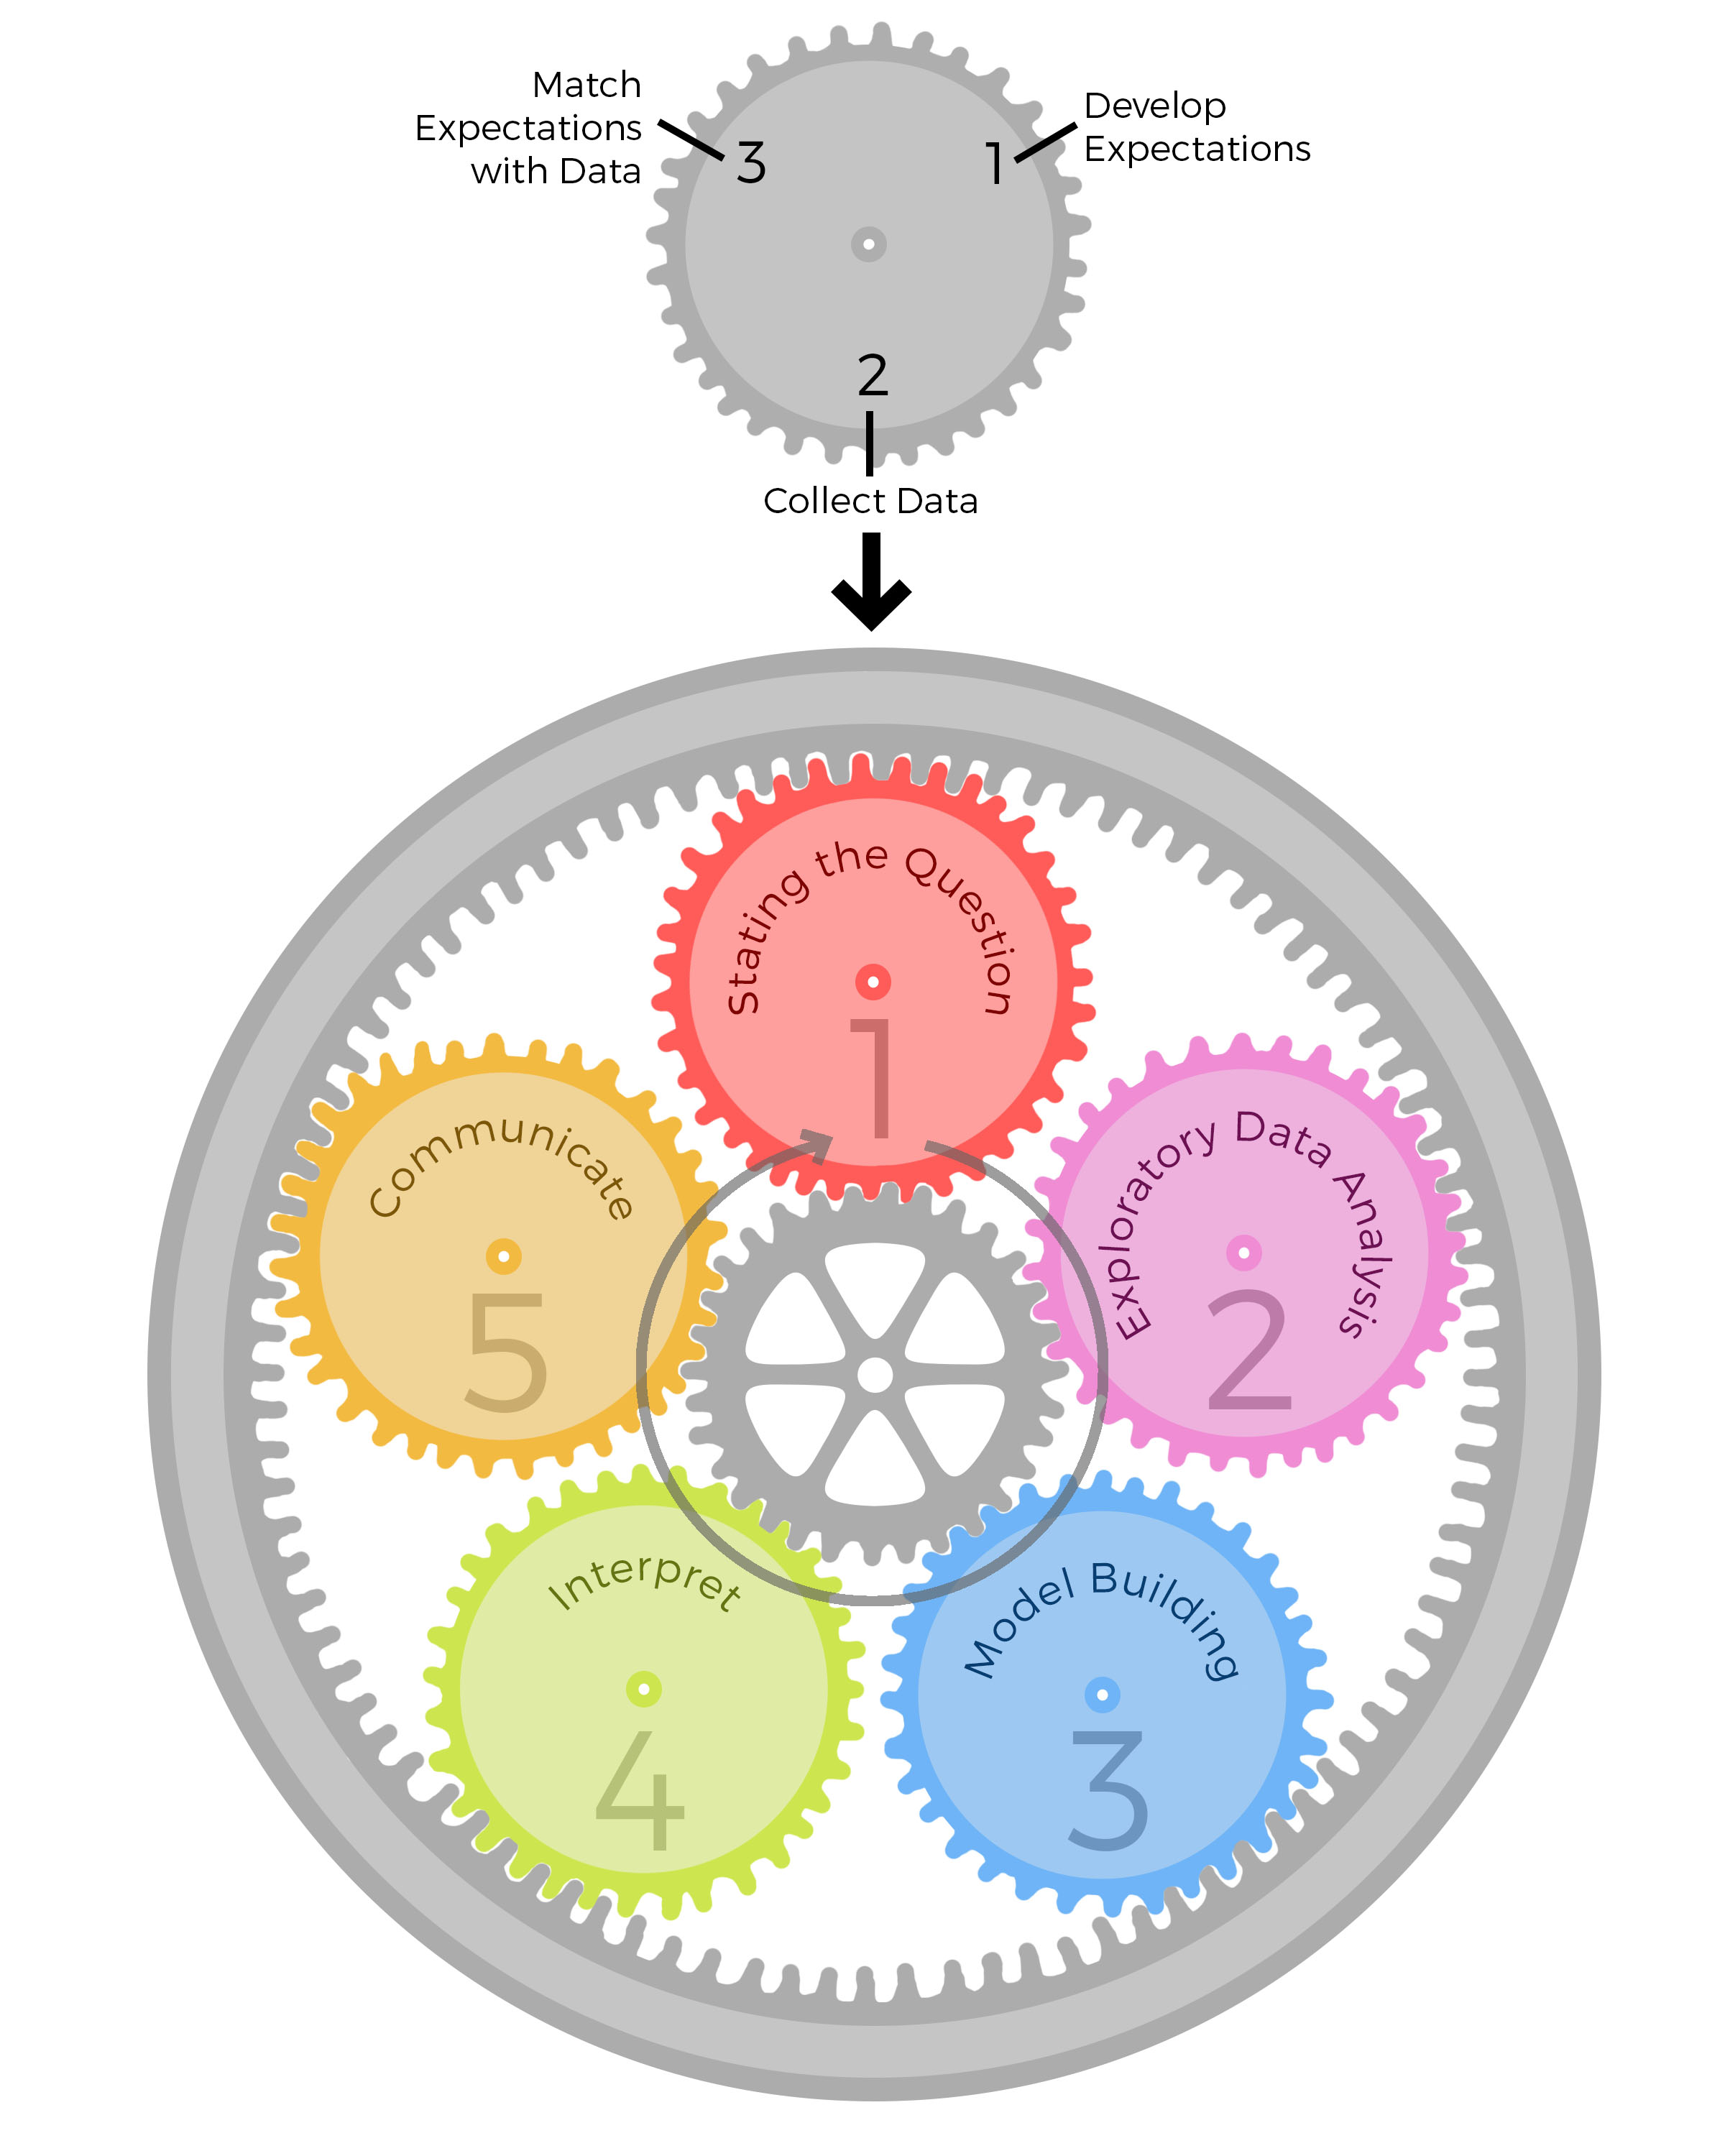
\includegraphics[width = 3in]{epicycle.png}
    \caption{Modelo de Epiciclos de Análisis de Datos (Fuente Peng y Matsui, 2017)}
\end{figure}

\subsection{Tareas Comunes en la Ciencia de Datos}
Hemos hablado de la ciencia de datos y su carácter predictivo. Las tareas mas comunes para lo cual se utiliza la ciencia de datos son las siguientes.

\begin{itemize}
	\item \textbf{Clasificación:} Decidir si algo pertenece a una categoría u otra. Harrington define la clasificación como la tarea de predecir a que tipo de clase pertenece una instancia (ejemplo) de la data propia de los métodos supervisados \cite{harrington}.
	\item \textbf{Puntuación:} Predecir o estimar un valor numérico, tal como lo es un precio o la probabilidad de un fenómeno. Alpaydin define esto como la extracción de reglas de los datos de los cuales se puede esperar estadísticamente un comportamiento similar y por lo cual se pueden efectuar predicciones correctas para instancias nuevas \cite{alpaydin}.
	\item \textbf{Ranking:} Aprender a ordenar objetos por preferencias
	\item \textbf{Agrupamientos:} Agrupar objetos en grupos de características homogéneas. Las técnicas de agrupamiento son típicas de los métodos de aprendizaje automatizado no-supervisados, donde en vez de buscar clasificar en clases conocidas o puntuar con valores ciertos, se busca la características comunes de la data para la agrupación de la misma en clases, tomando en cuenta que dichas clases no son conocidas a priori \cite{harrington}. 
	\item \textbf{Relaciones:} Encontrar relaciones o causas potenciales de efecto tal cual se ven en la data. Para Alpaydin la regresión lineal es un perfecto ejemplo de búsqueda de relaciones en la ciencia de datos, donde existe una función con un juego de parámetros asociados $y = g(x \mid \theta)$, $g(.)$ es el modelo y $\theta$ son sus parámetros. $Y$ es un número dentro de una regresión y $g(.)$ es la función de la regresión \cite{alpaydin}
	\item \textbf{Caracterizaciones:} Utilización general de visualizaciones y reportes de la data. Un ejemplo notable lo da Witten y Frank al referirse a la técnica de \emph{Market Basket Analysis} dentro de la mercadotecnia \cite{datamining}. En dicha técnica se busca que otros artículos comprarán los consumidores basados en el comportamiento registrado de sus compras pasadas. En términos matemáticos, estamos buscando $P(Y \mid X,D) = x_i$ donde $D$ es el juego conocido de datos históricos de los movimientos comerciales de los consumidores. 
\end{itemize}

\section{Aprendizaje Automatizado}
El aprendizaje automatizado es un campo de la ciencia de la computación donde se busca darle a las computadores la habilidad de aprender sin ser explicitamente programadas. El término se le atribuye a \textbf{Arthur Samuel}, un pionero del campo de la inteligencia artificial, qui	en lo acuñó en 1959 (Kohavi, R. y Provost, F., 1998). 

Es interesante que los métodos de aprendizaje automatizado proliferaron de forma paralela al concepto de ciencia de datos, y solo fueron absorbidos por esta en los últimos diez años. Alpaydim nos describe el aprendizaje automatizado como la programación de computadoras para optimizar un criterio de desempeño utilizando datos o experiencia pasada (Alpaydim, E., 2010). Tom Mitchell respeta este concepto al describir el aprendizaje automatizado como "\ldots la construcción de programas computacionales que aprenden con la experiencia\ldots” (Mitchell, T., 1997, pág. XV). Solo Peter Harrington utiliza una descripción mucho más simplista al determinar que “El aprendizaje automatizado es la extracción de información de la data.” (Harrington, P. 2012, pág. 5). 

Estudiar los procedimientos de aprendizaje automatizado equivale a estudiar tres temas principales que los componen.

\begin{itemize}
	\item Diseño del estudio: conjuntos de entrenamiento y conjuntos de predicción
	\item Problemas conceptuales: error fuera de la muestra, curvas ROC
	\item Implementación práctica: en este caso en particular, un tema que se cubrirá con la biblioteca Caret
\end{itemize}

Todo el mundo predice todo tipo de aseveraciones, desde el resultado de una elección presidencial hasta el partido de fútbol del domingo de una liga en particular. Pero en el sentido estricto de la palabra, ¿qué significa predecir? En nuestro contexto científico, definiremos el acto de predecir como el resultado de utilizar la probabilidad y muestreo para la selección de un conjunto de entrenamiento, el cual utilizaremos para construir las características de diseño de una función de predicción. La función utilizará dichas características para generar nuevas predicciones.  Los componentes para la selección adecuada de variables de predicción son los siguientes:

TO DO: Agregar el siguiente esquema
Pregunta > Datos > Atributos > Algoritmo > Parámetros > Evaluación

Un ejemplo muy común utilizado generalmente para explicar el uso del aprendizaje automatizado es la detección de correo chatarra, también conocido como spam. Podemos utilizar atributos cuantitativos de los mensajes, por ejemplo la frecuencia de ciertas palabras, para que un modelo se entrene y pueda predecir dentro de ciertos rangos de certeza si un correo cualquiera es o no spam. 

\subsection{Importancia Relativa de Los Pasos}

Hay una secuencia de pasos importante para la consecución de modelos de aprendizaje automatizado coherentes.

TO DO: Agregar el siguiente esquema como gráfico
Pregunta : Data : Atributos : Algoritmos

La combinación de algunos datos y un deseo extremo de conseguir una respuesta no nos asegura que una razonable pueda extraerse de un cuerpo cualquiera de información (Tukey, 1977). También es útil recordar que la calidad de los datos que ingresan al conjunto de entrenamiento tienen un efecto sobre el resultado del modelo. Datos que no son útiles no aportan nada. Es mucho mejor que la data sea curada y organizada de manera que tenga alta relevancia al tema de estudio. 

Los buenos atributos son aquellos que comparten las siguientes características:

\begin{enumerate}
	\item ayudan a comprimir la data
	\item retienen el mayor volumen de información relevante
	\item son creados basados en un modelo experto del modelo a aplicarse
\end{enumerate}

No es fácil hacer una buena selección de atributos que mas adelante se convertirán en variables de predicción. Los errores mas comunes son los siguientes. 

\begin{enumerate}
	\item tratar de automatizar la selección de atributos
	\item no prestar la atención necesaria a las variaciones y particularidades de los datos
	\item desechar información importante innecesariamente
\end{enumerate}

En este sentido los algoritmos importan mucho menos que la selección y curación de la data a utilizar. Los mejores métodos de aprendizaje automatizado reúnen una serie de características que los hace justamente sobresalir del montón. Las características en mención son las siguientes:

\begin{enumerate}
	\item Interpretable: 
	\item Simples:
	\item Precisos:
	\item Rápidos (de entrenar y evaluar):
	\item Escalables: 
\end{enumerate}

La predicción de modelos se basa mucho en el arte de compensar beneficios versus necesidades.

\begin{enumerate}
	\item interpretación de los datos vs. precisión
	\item velocidad vs. precisión
	\item simplicidad vs. precisión
	\item modelos escalables vs. precisión 
\end{enumerate}

A pesar de tener que sopesar la mejor forma de compensar todas estas variables, la interpretación es muy importante y debe conservar su lugar, ya que poco sirve un modelo rápido y preciso que no se puede interpretar. Muchos autores otorgan un segundo lugar de importancia a lo escalable del modelo. Se han dado casos donde modelos muy precisos no se han podido poner en producción por la complejidad de escalar el algoritmo. El caso mas mencionado es el premio NETFLIX, el cual otorgo un millón de dolares al equipo con el mejor modelo de predicción de gustos de sus clientes, solo para luego llegar a la conclusión que el mismo era demasiado complejo y lento de escalar en producción y archivarlo (Techdirt, 2012).

\subsection{Métodos Supervisados y No-Supervisados}
Para los autores Hastie, Tibshirani, y Friedman el aprendizaje supervisado intenta aprender una función f de predicción a través del uso de uso juegos de datos de entrenamiento en forma de muestras del total de los datos disponibles. El uso de datos de entrenamiento le permite al sistema aprender y minimizar el error del modelo de predicción \cite{theElements}.  

Harrington nos da una explicación más sencilla del término, al aclarar que el aprendizaje supervisado es aquel que le pide al computador aprender de los datos utilizando una variable específica como objetivo. Esto reduce la complejidad de algoritmos y patrones que se deben derivar de la muestra de datos \cite{harrington}. 

El profesor Alpaydin agrega que el aprendizaje supervisado tiene como objeto aprender un mapeo de los elementos de entrada a los de salida, teniendo en cuenta que los valores correctos de estos últimos están dados por el supervisor \cite{alpaydin}.

\subsection{Error Muestral y Error Fuera de Muestra}
El siguiente concepto es fundamental dentro de la teoría de aprendizaje automatizado, y la terminología puede diferir un poco de los términos establecidos en la estadística inferencial.

	\begin{itemize}
		\item \textbf{Error dentro de la muestra:} es el margen de error que se obtiene al utilizar el juego de datos de entrenamiento en la construcción del modelo de predicción. También se conoce como error de re-substitución 
		\item  \textbf{Error fuera de muestra:} es el margen de error que se obtiene cuando se aplica el modelo de predicción a un nuevo juego de datos. También se lo conoce como error de generalización. 
	\end{itemize}


En este punto debemos aclarar cuales son las ideas principales en las que hay que enfocarse. 

\begin{enumerate}
	\item Principalmente estamos interesados mucho mas en el error de generalización - el que se obtiene al aplicar un nuevo juego de datos al modelo de predicción - que del margen de error de resubstitución.
	\item El error de resubstitución siempre va a ser menor que el error de generalización 
	\item La razon por la cual se da este fenómeno (que el error de resubstitución sea menor que el error de generalización) es el efecto de sobreajuste. El algoritmo se está ajustando de más a los datos.
\end{enumerate}

La data en la ciencia de datos tiene dos partes: señal y ruido. El objetivo del modelo de predicción es el de predecir la señal. Siempre se puede diseñar un modelo perfecto que capture tanto la señal como el ruido. Pero dicho modelo no se desempeñará bien en juegos de datos nuevos. 

El efecto de sobreajuste se como la creación de un modelo optimista a partir del juego de datos de entrenamiento. Los métodos que utilizamos buscan interpretar los datos de tal manera que no solo se ajustan a la señal sino al ruido de los mismos. Por esa razón el margen de error de resubstitución (error dentro de la muestra) es tan bajo pero cuando se prueba el mismo modelo entrenado en un juego de datos externo el margen de error generalizado (fuera de la muestra) crece. Se ha comprobado que los errores por sobreajuste ocurren más en modelos complejos que en modelos sencillos. La razón es que muchas veces el modelo complejo es precisamente más complicado para ajustarse mejor a la señal de los datos, sin que estos ajustes sean necesarios - o precisos - al momento de cambiar del juego de datos. 

\subsection{Diseño de un Estudio de Aprendizaje Automatizado}
El diseño de una investigación de ciencia de datos tiene seis pasos. El diseño del estudio de un problema de aprendizaje automatizado debe verse como el diseño de la fase de modelo (paso tres) mucho más detallado para no confundirlos. La metodología recomendada por el Dr. Jeff Leek (Leek, J. 2015) recomienda los siguientes seis:

\begin{enumerate}
	\item Definir el margen de error deseado
	\item Dividir la data en juegos específicos de entrenamiento, evaluación y validación (opcional)
	\item En el juego de entrenamiento, seleccionar atributos y utilizar validación cruzada
	\item En el juego de entrenamiento, seleccionar la función de predicción; utilizar nuevamente validación cruzada
	\item si no se utilizo validación cruzada, aplicar prueba 1X al juego de evaluación
	\item si se utilizo validación cruzada, aplicar prueba al juego de evaluación, refinar el algoritmo, y luego volver a someter 1X al juego de validación 
\end{enumerate}

A pesar de que no tiene una comprobación científica, la comunidad siempre aconseja evitar las muestras pequeñas de la misma forma que se evitan en la estadística clásica. Una pregunta válida es cuanto de los datos disponibles se deben destinar al juego de entrenamiento, cuantos al juego de validación y cuantos al juego de evaluación. Zumel y Mount (Zumel, N., Mount, J., 2014) consideran un modelo sencillo de división con 90\% de los datos destinados al entrenamiento de modelos y el 10\% restante a la evaluación. Sin embargo Leek (Leek, J. 2015) en su libro \emph{Data Style} nos da un juego de reglas mas comprensivas de como distribuir los datos segun el volumen de los mismos. 

\textbf{A. Si el volumen de datos es grande}
\begin{itemize}
	\item 60\% para el juego de entrenamiento
	\item 20\% para el juego de evaluación
	\item 20\% para el juego de validación 
\end{itemize}

\textbf{B. Si el volumen de datos es mediano}
\begin{itemize}
	\item 60\% para el juego de entrenamiento
	\item 40\% para el juego de evaluación
\end{itemize}

\textbf{C. Si el volumen de datos es pequeño}
\begin{itemize}
	\item entrenar sobre el 100\% de los datos
	\item utilizar validación cruzada sobre el mismo juego que se entrenó
	\item no ocultar el hecho hacer alusión en la investigación de la muestra poco representativa
\end{itemize}

La tentación de utilizar el juego de datos de validación y/o evaluación es muy grande para todos los científicos de datos noveles. Sin embargo la literatura concuerda en que no se debe utilizar la evaluación sino hacia el final del proceso. 

La selección de que datos en particular deben elegirse en cada grupo debe ser aleatoria, con un porcentaje definido en cada uno pero total certeza de que no hay parcialidad en la selección. En el caso del lenguaje R, la biblioteca CARET tiene incorporada funciones para garantizar asignaciones de datos a los grupos de entrenamiento y evaluación totalmente aleatorios. Los juegos finales de datos deben reflejar sin embargo las mismas estructuras del problema. Un claro ejemplo son las series de tiempo (Hyndman, R., 2012) en las cuales los datos tiene un componente de tiempo que denota un orden en especial. De estos grupos debe seleccionarse muestras aleatorias pero representativas de los periodos de tiempo a fin de tener sentido. A su vez cada sub-muestra debe reflejar el mayor grado de diversidad posible. Esto se debe lograr con selección aleatoria pero a veces es difícil mantener dicho balance con la mezcla posible de atributos.

\subsection{Tipo de Errores}
El concepto de error en estadística es uno que embarca varias dimensiones. En lo que respecta al aprendizaje automatizado, no importa que tan grande sea la muestra ni que tan exacto sea el algoritmo, siempre cabe la probabilidad - aunque pequeña - que una predicción sea falsa a pesar de que arroja un resultado positivo. Podemos entonces dividir los tipos de errores según su predicción y verdadera naturaleza (Yakir, B. 2011). 

En lineas generales diremos que un resultado es positivo si ha sido identificado como tal, y que es negativo si ha sido rechazado. De tal forma:
\begin{itemize}
	\item \textbf{verdadero positivo:} es aquel que ha sido correctamente identificado
	\item \textbf{falso positivo:} es aquel que ha sido incorrectamente identificado
	\item \textbf{verdadero negativo:} es aquel que ha sido correctamente rechazado
	\item \textbf{falso negativo:} es aquel que ha sido incorrectamente rechazado
\end{itemize}

La combinación de los siguientes resultados nos permite medir estadísticamente variables pertinentes a los resultados del modelo. Estas variables se conocen como sensibilidad, especificidad, valor predictivo positivo, valor predictivo negativo, y exactitud.

\textbf{Sensibilidad:} La sensibilidad es la probabilidad que un fenómeno arroje un valor positivo cuando realmente lo es. Por ejemplo, un examen de una enfermedad da positivo cuando el paciente realmente esta enfermo de dicho padecer. Podemos expresar la formula como un cociente de la siguiente forma:

\begin{equation}
sensibilidad = \frac{VP}{(VP + FN)}
\end{equation}

\textbf{Especificidad:} La especificidad es la probabilidad que un fenómeno arroje un valor negativo cuando realmente no se encuentra presente (o sea es una predicción negativa cuando la realidad también es negativo). Por ejemplo, un examen de embarazo que da negativo cuando la paciente no esta embarazada. Podemos expresar la formula como un cociente de la siguiente forma:

\begin{equation}
especificidad= \frac{VN}{(FP + VN)}
\end{equation}

\textbf{Valor Predictivo Positivo:} El valor predictivo positivo es la probabilidad de que un fenomeno este presente cuando la predicción arroja un valor positivo. Por ejemplo, la probabilidad de que un paciente tenga diabetes cuando el examen arroja positivo. Podemos expresar la formula como un cociente de la siguiente forma:

\begin{equation}
\mbox{\textit{valor predictivo positivo}} = \frac{VP}{(VP + FP)}
\end{equation}

\textbf{Valor Predictivo Negativo:} Lo opuesto del valor predictivo positivo, es la probabilidad de que una prediccion arroje negativo cuando el fenómeno no este presente. Por ejemplo, la probabilidad de que un paciente no se le detecte diabetes cuando en la vida real no la tiene. Podemos expresar la formula como un cociente de la siguiente forma:

\begin{equation}
\mbox{\textit{valor predictivo negativo}} = \frac{VN}{(VN + FN)}
\end{equation}

\textbf{Exactitud:} Quizás el mas sencillo de percibir de forma natural, la exactitud es simplemente la probabilidad de una prediccion correcta. Podemos expresar la formula como un cociente de la siguiente forma:

\begin{equation}
exactitud = \frac{VP + VN}{(VP + FP + VN + FN)}
\end{equation}

\subsubsection{Midiendo Error en Data Continua}
Para data continua, de naturaleza numérico, las dos formas de medir el error mas comunes en aprendizaje automatizado son el error cuadrático medio y la raíz error cuadrático medio. 

La raíz error cuadrático media es utilizada con frecuencia para medir la diferencia entre valores (de una muestra y valores de una población) predicha por un modelo o un estimador y los datos observados en la realidad. Este valor representa la desviación estándar de la muestra entre los valores predecidos y los valores observados. Las diferencias individuales entre estas dos medidas se conocen como residuos si son extraídos de la muestra, y errores de predicción si son calculados fuera de muestra. 

\begin{equation}
\sqrt{\frac{1}{n}\sum_{i=1}^n(prediccion_{i} - observado_{i})^{2}}
\end{equation}

\subsection{Sobreajuste}
En aprendizaje automatizado, el sobreajuste (también es frecuente emplear el término en inglés overfitting) es el efecto de sobre-entrenar un algoritmo de aprendizaje con unos ciertos datos para los que se conoce el resultado deseado. Daroczi define el sobreajuste como la descripción del modelo en conjunto con el ruido aleatorio de la muestra en vez de solo el fenómeno generador de datos \cite{daroczi}. El sobreajuste ocurre, por ejemplo, cuando el modelo tiene más predictores de los que puede acomodar la muestra de datos.

Según Zumel y Mount, una de las señales de sobreajuste más sencillas de detectar se da cuando un modelo tiene un excelente desempeño en el juego de datos que se entrenó, pero uno muy malo en un juego de datos nuevo \cite{zumelMount}. Esto es causa y efecto de memorizar la data de entrenamiento en vez de aprender reglas generales de la generación del patrón. 

\subsection{R y la Biblioteca CARET}
La biblioteca \emph{CARET} (nombre extraído de Classification And Regression Training) es una libreria de funciones en R para optimizar el proceso de crear modelos predictivos. El paquete contiene herramientas para:

\begin{itemize}
	\item segmentar juegos de datos
	\item preproceso de los datos
	\item seleccion de predictores
	\item optimizacion del modelo utilizando reconfiguracion de muestras
	\item estimacion de la importancia de la variable
\end{itemize}

El paquete esta mantenido en GitHub bajo la administración del Doctor en Estadística Max Kuhn. 

\section{Modelos Ensamblados}
El tema de modelos ensamblados es uno que por lo general se reserva más como técnica de composición que cómo teoría del aprendizaje automatizado. Los modelos ensamblados ayudan a mejorar los resultados del aprendizaje automatizado combinando diferentes modelos. Este enfoque permite la producción de mejores modelos predictivos en contraposición a la utilización de un solo modelo \cite{smolyakov}.

\subsection{Introducción}
  El uso de modelos ensamblados es en cierta forma la prueba final de la hipótesis de trabajo: la utilización de dos modelos entrecruzados cuyos resultados conforman una tabla temporal de valores esperados de los cuales se genera un nuevo modelo sintético de predicción más general y con mayor capacidad de predicción en juegos de datos de validación cruzada. Este concepto es novel; Witten y Frank lo describen como combinación de métodos múltiples, y escriben: “… un enfoque obvio para hacer mejores decisiones es tomar el resultado de diferentes métodos y combinarlos\ldots” \cite{datamining}. Zhou nos describe que “… los modelos ensamblados que entrenan múltiples variables y luego las combinan para uso de entrenamiento, con el Boosting y el Bagging como representantes principales, representan lo más novedoso en el estado del arte de la ciencia de datos…” \cite[p. 7]{ensembleMethods}. De una manera un tanto más coloquial, Zhang y Ma describen el uso de modelos ensamblados con una analogía de la vida real, en la cual los pacientes buscan una segunda y hasta tercera opinión de expertos antes de someterse a una operación complicada \cite{ensembleMachineLearning}. Curiosamente tanto Zhang, Ma y Zhou hablan de la combinación de métodos de regresión general con clasificadores, y solo Witten y Frank hablan de otras combinaciones (por supuesto, Witten y Frank comenzaban a escribir en los albores del ensamblaje de métodos, cuando los clasificadores no estaban tan de moda porque el análisis era mayoritariamente de números, algo que cambió con el avance de las redes sociales). Una de las descripciones más sucintas y prácticas es la de Vadim Smolyakov, quien define el uso de modelos ensamblados como meta-algoritmos que combinan dos o más técnicas de aprendizaje automatizado en un modelo predictivo de forma que se logre disminuir la varianza (bagging), el sesgo (boosting) o se mejore la precisión (stacking) \cite{smolyakov}. 

\subsection{Combinando Métodos}
La combinación de métodos es el ultimo paso en la estrategia de construcción de un sistema ensamblado de aprendizaje automatizado. La pregunta de que métodos combinar esta estrechamente relacionado con el tipo de juegos de datos y la solución que se busca alcanzar. Por ejemplo, alguno métodos de clasificación como los vectores de soporte solo devuelven valores discretos \cite{ensembleMachineLearning}. De tal manera el uso de dos métodos alternos en uno ensamblado estará determinado por la forma final en que se ensamblan y el algoritmo final utilizado para la decisión de predicción. Tanto Polikar \cite{ensembleMachineLearning} como Zhou \cite{ensembleMethods} citan como preferibles las metodologías de voto por mayoría, promedio, promedio ponderado, y ensamblaje infinito. Dzeroski y Zenko denotan que la mayoría de la investigación alrededor de métodos ensamblados se da con la generación de ensambles utilizando un único algoritmo de clasificación, como por ejemplo los árboles de decisión o el entrenamiento de redes neuronales \cite{DzeroskiZenko}. 

Smolyakov divide los métodos ensamblados en dos grandes clasificaciones \cite{smolyakov}:

\begin{itemize}
  \item \textbf{Métodos Ensamblados Secuenciales:} son aquellos donde los modelos bases de aprendizaje se generan de forma secuencial. La idea inicial es que se explota la dependencia entre dichos modelos base al momento de generarlos. Un buen ejemplo de modelos ensamblados secuenciales es \emph{AdaBoost}. El desempeño de predicción o la acotación del margen de error se optimiza al calibrar los regresores y/o clasificadores después de cada entrenamiento y previo al próximo. 
  \item \textbf{Métodos Ensamblados Paralelos:} son aquellos en los cuales los modelos bases se generar en forma paralela e independiente. Un buen ejemplo de modelos ensamblados paralelos es \emph{Random Forest}. La motivación de utilizar modelos ensamblados paralelos es maximizar la independencia entre los regresores y/o clasificadores que se optimizan entre si al promediar los resultados, reduciendo el margen de error. 
\end{itemize}

\subsection{Diversidad}
La diversidad de ensamblaje, o la diferencia entre diferentes métodos de aprendizaje, es un tema fundamental en el ensamblaje de métodos \cite{ensembleMethods}. Intuitivamente es fácil entender que para obtener una ventaja de la combinación, es necesario que los aprendizajes sean diferentes, de otra manera la ganancia en desempeño no seria marginalmente superior a los métodos por separado \cite{ensembleMethods}.

La mayoría de los métodos ensamblados utilizan solo un tipo de modelo base de algoritmo de aprendizaje para producir regresores o clasificadores homogéneos (del mismo tipo) conocidos como \textit{ensamblajes homogéneos} \cite{smolyakov}. También existen métodos que utilizan diferentes tipos de modelos bases como clasificadores y/o regresores. Estos modelos ensamblados se conocen como \textit{modelos heterogeneos}. Para poder ensamblar modelos más precisos que cualquiera de sus modelos base por si solos es necesario que los modelos bases sean precisos en primera instancia, y tan diversos como sea matemáticamente posible \cite{smolyakov}.

Para propósitos de este marco teórico revisaremos de forma breve los tres métodos más utilizados en la actualidad para el ensamblaje que son:
\begin{itemize}
  \item Bagging: cuando se busca reducir la varianza en los clasificadores
  \item Boosting: cuando se busca reducir el sesgo 
  \item Stacking: cuando se busca aumentar la predicción de los regresores
\end{itemize}

Dado que la hipótesis de trabajo del siguiente estudio utiliza el ensamblaje heterogéneo de modelos bases de regresión lineal y pronóstico de series de tiempo con ARIMA, haremos un alto para entrar con más detalle en la teoría y bondades de los modelos apilados (\emph{stacking}).

\subsection{Bagging}
La idea del \emph{bagging} esta estrechamente ligada al \emph{bootstrapping}, y determinada por la selección de múltiples muestras de datos generadas a través de \emph{bootstrapping}, utilizadas para alimentar clasificadores, sobre cuyos resultados el método ensamblado puede votar \cite{daume}. La palabra \emph{bagging} es la composición de \emph{bootstrap aggregation}. La etimología proviene de la metodología propia del método, que usa la agregación de múltiples muestras generadas de los datos disponibles (por ende, el \emph{bootstrapping}) para promediar múltiples estimados \cite{smolyakov}. 
Por ejemplo, se pudiera utilizar el \emph{bagging} para entrenar M árboles diferentes en diferentes juegos de datos seleccionados al azar con reemplazo para computar el ensamblado siguiente:  

\[ f(x) = \frac{1}{M} \sum_{m=1}^M f_m^{(x)} \]

\emph{Bagging} utiliza muestreo por \emph{bootstrap} para obtener juegos de datos para entrenar los modelos base. Para agregar los resultados de los modelos base, el \emph{bagging} utiliza dos maneras:
\begin{enumerate}
  \item votación para clasificadores
  \item promedios para regresión
\end{enumerate}

\subsection{Boosting}
El \emph{boosting} se refiere a una familia de técnicas de algoritmos que tienen la capacidad de convertir clasificadores (o regresores) débiles en entrenadores fuertes. El principio del \emph{boosting} es calzar una secuencia de clasificadores débiles - modelos que son escasamente mejores en la predicción que selección al azar, como por ejemplo pequeños árboles de decisión - a versiones ajustadas y sopesadas de los datos. Más peso se le otorga a los clasificadores que fueron mal clasificados en rondas anteriores \cite{smolyakov}. Daume describe el método como "\ldots La forma en la cual funciona el \emph{boosting} es que basado en un juego de datos y resultados pasados, va generando nuevas predicciones. Las predicciones con resultados aceptables se les pone menor peso y recursos, mientras que el algoritmo vuelve a iterar en aquellas predicciones con valores lejanos hasta que cobran fuerza \ldots" \cite{daume}. Esta técnica recibe el nombre de \textbf{AdaBoost}, del ingles \emph{adaptive boosting algotithm}. \textbf{AdaBoost} fue una de las primeras técnicas practicas en la ciencia de datos.

Los algoritmos de \emph{AdaBoost} comienzan ajustando los pesos del clasificador base \(y_1(x)\) a \(\frac{1}{N}\). Al comienzo todos los coeficientes de peso son los mismos. En rondas subsiguientes los coeficientes de peso se aumentan para aquellos puntos de datos que han sido mal clasificados y se reduce el peso de aquellos que han sido clasificados correctamente. Esta iteración es la que permite fortalecer los clasificadores débiles (a la vez fortaleciendo los débiles y debilitando los fuertes para contrastar mejor) \cite{smolyakov}. 

Existe una variable epsilon que representa el error ajustado de cada clasificador base. Hacia el final de las iteraciones del algoritmo los coeficientes ajustados alfa le otorgan mayor peso a los clasificadores con mayor precisión (la cual ha sido ajustada en \(n\) iteraciones). 

Una metodología derivada es el \emph{Boosting de Árboles Degradados}. Dicho método es una generalización del \emph{boosting} para funciones arbitrarias de pérdida \cite{smolyakov}. El mismo se puede utilizar tanto para problemas de clasificación como de regresión, y construye el modelo de forma secuencial:

\[ F_m(x) = F_{m-1}(x) + \gamma_m^{h_m(x)} \]

En cada nodo del árbol de decisión \(h_m(x)\) se elige para minimizar una función de pérdida \(L\) dado el modelo actual \(F_{m-1}(x)\):

\[ F_m(x) = F_{m-1}(x) + \argmin_h \sum_{i=1}^n L(y_i, F_{m-1}(x_i) + h(x_i) )\]

Los algoritmos para regresión y clasificación en este caso utilizan diferentes tipos de funciones de pérdida cuya explicación queda fuera del alcance de este marco teórico. 

\subsection{Stacking}
El \emph{stacking} - del inglés apilar - es una técnica de aprendizaje ensamblado que combina múltiples modelos de regresión o clasificación mediante un meta-regresor o un meta-clasificador. Los modelos base se entrenan en el juego de datos de entrenamiento, y luego el meta-modelo es entrenado en los resultados de los modelos base como variables \cite{smolyakov}. Los modelos base por lo general son diferentes algoritmos de aprendizaje automatizado, por lo que los modelos ensamblados por \emph{stacking} son usualmente heterogéneos. David Wolpert, del Centro de Estudio de Los Alamos, Nuevo México, escribió por primera vez sobre el método. Su propuesta era utilizar stacking generalizado como una manera de reducir el sesgo del entrenamiento de datos y el error de generalización. La tesis planteada es que el \emph{stacking} tiene un mejor margen de generalización ya que reduce el mismo al utilizar como fuente de datos de entrenamiento las predicciones (el cual denomina conjeturas en su artículo original) de un juego inicial de clasificadores \cite{wolpert}. Wolpert habla de un aprendizaje automatizado en dos espacios, uno inicial donde se toma como entradas los clasificadores base, y un segundo espacio, donde bautiza como \emph{generalizador} lo que la literatura actual denomina el meta-clasificador. La idea de generalización era la reducción del error del modelo aplicado a la vida real en solución de problemas. El concepto de sobreajuste (\textit{overfit}) no figura entonces pero lo que se buscaba era un método que generalizara mejor sobre datos de validación reduciendo el error generado por el sobreajuste de los modelos base sobre el juego de datos de entrenamiento. Dzeroski y Zenko han continuado los estudios de Wolpert y han presentado nuevos métodos de \emph{stacking}, incluyendo el uso de distribuciones de probabilidades y regresión lineal de múltiples respuestas como opciones que clasifican y predicen como mayor precisión \cite{DzeroskiZenko}. Ting y Witten definen la generalización por \emph{stacking} como una metodología general que utiliza un modelo de alto nivel que combina modelos inferiores para alcanzar mayores niveles de precisión en la predicción \cite{tingwitten}.

Dado que gran parte del trabajo de tesis doctoral involucra el uso de \emph{stacking}, el pseudo-código para el algoritmo se presenta a continuación. \\

\begin{lstlisting}
Input: data entrenamiento D = {xi,yi}, i=1...m
Output: clasificados ensamblado H
Paso 1: aprender de los clasificadores base
para t = 1 a T hacer:
	aprender h(t) basado en D
terminar bucle
Paso 2: construir un nuevo juego de datos para predicciones
para i = 1 a m hacer:
	D(h) = {xi', yi}, donde xi' = {h1(xi), ..., hT(xi)}
terminar bucle
Paso 3: aprender del meta-clasificador
aprender H basado en D(h)
retornar H
\end{lstlisting}

Entrando en mayor profundidad sobre la metodología, el \emph{stacking} se centra en la combinación de múltiples clasificadores generados por la utilización de diferentes algoritmos $L_1, \ldots, L_N$ en un juego de datos único S, el cual consiste de ejemplos $s_1 = (x_i, y_i)$, pares de vectores $(x_i)$ y sus clasificaciones $(y_i)$. En la primera fase, un juego de clasificadores bases $C_1, C_2, \ldots, C_N$ se generan, donde $C_i = L_i(S)$. En la segunda fase, un meta-clasificador se aprende de la combinación de salidas del clasificador base \cite{wolpert}

Para generar un juego de entrenamiento para el meta-clasificador, se puede aplicar un proceso de \emph{validación cruzada} o \emph{dejar-uno-fuera}. En caso de utilizar el proceso de dejar-uno-afuera, se aplica cada uno de los algoritmos base a todo el juego de datos menos un ejemplo para prueba: $\forall i = 1, \ldots, n : \forall k = 1, \ldots, N : C^{i}_{k} = L_k(S - S_i)$. Luego se utilizan los clasificadores aprendidos para generar predicciones para $s_i : \hat{y}^{k}_{i} = C^{i}_{k}(x_i)$. El juego de datos a meta-nivel consiste de ejemplos de la forma $((\hat{y}^{l}_{i}, \ldots, \hat{y}^{n}_{i}), y_i)$ donde los regresores o clasificadores son las predicciones de los regresores/clasificadores base y la clase es la clase correcta del ejemplo a mano \cite{DzeroskiZenko}.

La decisión de que meta-clasificador o meta-regresor utilizar es por el momento decisión del científico de datos en cada caso, y un tema que ha llevado a controversias en la comunidad de la ciencia estadística.  El método de stacking continúa su evolución como por ejemplo el uso de distribuciones de probabilidades. Ting y Witten continúan el trabajo de Wolpert concentrandosé en los que ellos llaman los dos factores cruciales de los métodos de \emph{stacking} generalizado: el tipo de generalizador más conveniente para derivar el modelo de nivel superior, y los tipos de atributos que debieran ser utilizados como variables de ingreso \cite{tingwitten}. Los autores introducen una metodología novel donde se ensamblan clasificadores cuyas predicciones son las distribuciones de probabilidad de los valores de las clases, en vez de los valores de las clases en si. Ende, los meta-atributos son probabilidades de cada una de los valores de clase que arroja cada uno de los clasificadores base. Los autores aducen que esto no solo les permite hacer predicciones, sino utilizar el intervalo de confidencia de los clasificadores base. 

Cada clasificador base predice una distribución de probabilidades para un juego de posibles valores de clase. La predicción de un clasificador base $C$ aplicada al ejemplo $x$ es una distribución de probabilidades a su vez:

\[ p^c(x) = (p^c(c_1 \mid x), (p^c(c_2 \mid x), \ldots, (p^c(c_m \mid x)) \]

donde ${c_{1}, c_{2}, \ldots, c_m}$ es el rango de posibles valores de la clase y $(p^c(c_i \mid x)$ denota la probabilidad de que dicho ejemplo $x$ pertenezca a la clase $c_i$ como lo estima (y predice) el clasificador $C$. La clase $c_j$ con la probabilidad más alta $p^C(c_j \mid x)$ se predice con el clasificador $C$. Los meta-atributos son las predicciones de probabilidades para cada clase posible según cada uno de los clasificadores base \cite{DzeroskiZenko}. 

\subsection{Marco Conceptual}
La TRM representa un ejemplo perfecto de series de tiempo con marcada tendencia secular y estacionalidad. Pudiéramos en cualquier caso utilizar métodos de pronóstico de series de tiempo como ARIMA para entonces estimar el valor futuro de la TRM. Sin embargo, esta estimación tendría como único elemento de referencia el valor de la TRM en diferentes puntos del tiempo. Estaríamos resolviendo el problema haciendo caso omiso de las diferentes variables exógenas que intervienen en la economía mundial y de Colombia, y que juntas definen a través de la ley de oferta y demanda el valor final de la TRM.
 
En dicho caso, el uso de regresión lineal y regresión multivariable nos permite justamente crear un modelo de pronóstico basado en regresores relacionados con la variable independiente que a su vez son variables exógenas. A través de la creación de dicho modelo la predicción se hace sin tomar en cuenta que la TRM es una serie de tiempo y puede aportar en su descomposición factores importantes tales como la estacionalidad de la tendencia.
 
Si partimos del hecho de que la TRM es una serie de tiempos y puede ser estudiada como tal, y que además los diferentes rubros de exportación de la economía de Colombia aportan divisas que a través de la ley de oferta y demanda regulan en el mercado sus precios, es una admisión de que existen variables relacionadas, aunque exógenas que rigen el comportamiento de la TRM además de sus tendencias seculares y estacionalidad.
 
Es válido, si partimos de ambos supuestos y los tomamos como ciertos, pensar que puede existir un modelo híbrido de pronóstico que tome en consideración ambos eventos. Hay claras sinergias entre las exportaciones de Colombia, fuentes de ingresos de divisas, que se manifiestan en indicios de comportamiento de cotización de mercado. Hay claras manifestaciones en la estacionalidad y tendencia de una serie de tiempos representativa de la TRM. Ambas metodologías de pronóstico son el reflejo de la realidad económica modelados de diferentes maneras.
 
La Ciencia de Datos utiliza el aprendizaje automatizado como forma de llegar a modelos complejos de clasificación y estimación. Es aprendizaje automatizado porque los datos son los que se entrenan y definen el modelo, no el científico. Si existen sinergias fuertes el modelo cobra vida de forma automática. Inclusive el aprendizaje automatizado prevé la existencia de modelos ensamblados, justamente para aumentar la capacidad de estimación cuando un fenómeno puede ser modelado mejor como una sumatoria de clasificadores y/o regresores que por un solo método. Por lo tanto, es plausible obtener un modelo de predicción de la TRM generado por el aprendizaje automatizado de series de tiempo y regresión multivariable en un solo método híbrido y ensamblado que parta desde:
 
\begin{itemize}
\item el uso de los valores de la TRM como serie de tiempo,
\item y los valores de la TRM y los diferentes rubros mayores que componen la canasta de exportación de Colombia como una estructura de datos para el análisis de regresión multivariable.
\end{itemize}

¿Cómo podemos predecir la TRM para mitigar el efecto negativo de las fluctuaciones en la tasa de cambio en la contabilidad de precios y costos?

La hipótesis de trabajo para resolver dicha pregunta postula un modelo basado en los principales rubros de exportación de Colombia diseñado con Machine Learning de los mismos datos:
\begin{itemize}
\item Existen una cantidad finita - e inferior a la decena - de productos de exportación que fungen como variables de agregación al producto bruto interno de Colombia y que son necesarias para la consecución de un modelo predictivo parsimonioso de la TRM.
\item El valor de la TRM, tal cual lo ja la Superintendencia Financiera de Colombia, no es sino el reflejo de los movimientos de estas variables de aportación que ayudan a modelar y controlar la tasa de cambio.
\item El comportamiento pasado de dichas variables puede ser utilizado para entrenar y generar un modelo estadístico predictivo parsimonioso utilizando aprendizaje automatizado cuyo margen de error sea inferior al 5\% (o, en otros términos, p < 0,05).
\item El modelo final no es único sino es el resultado del ensamblaje de varios modelos matemáticos predictivos y dinámico en su concepción ya que puede ser afectado por la acumulación de nuevos datos de retroalimentación a posteriori 
\end{itemize}

En términos formales:

\[ p^{c}(x) = (p^{c}(c_{1} \mid x),p^{c}(c_{2} \mid x)) \]

Donde:

\[ c_{1} : f(y) = \beta_{0} + \beta_{1}x_{1} + \beta_{2}x_{2} + \cdots + \beta_{n}x_{n} + \epsilon \]
\[ c_{2} : f(y_{t}) = \beta_{0} + \beta_{1}x_{t-1} + \beta_{2}x_{t-2} + \cdots + \beta_{n}x_{t-n} + \epsilon_{t}\]

En términos coloquiales, el modelo de predicción está determinado por el ensamblaje acumulado de dos clasificadores (ambos regresores), un modelo de regresión lineal y otro de pronóstico ARIMA.

La hipótesis de trabajo propuesta tiene marcada diferencias con los trabajos de otros investigadores en el área de predicción del FOREX. 

\begin{itemize}
\item Los investigadores Mehreen Rehman, Gul Muhammad Khan y Sahibzada Ali Mahmud han utilizado la ciencia de datos para la predicción de FOREX. Los autores utilizan CGP (Programación Genética Cartesiana), una extensión del uso de redes neuronales, para obtener predicciones del dólar australiano (Rehman, M., Khan, G. y Mahmud, S., 2014). Este modelo se alimenta exclusivamente de datos históricos de la cotizaciones de la moneda y no tiene datos de variables exógenas como los regresores propuestos de los rubros de exportación de Colombia. 
\item El estudio de los doctores Hossein Talebi, Winsor Hoang y Marina Gavrilova busca la mejora de sistemas automatizados de corretaje de FOREX. Los autores proponen un nuevo método de clasificación con extracción de clasificadores de múltiples escalas para el entrenamiento de datos, y luego se ensamblan diferentes clasificadores por voto Bayes (Talebi, H., Hoang, y Gavrilova, M., 2014). El trabajo tiene en cuenta el uso de métodos ensamblados pero utiliza como clasificadores pares de cotizaciones de monedas (por ejemplo el par COP:USD) las cuales pueden pensarse como un ensamble de dos series de tiempo sin uso de variables exógenas. 
\item Los profesores de matemática de la universidad de Beijing Lean Yu, Shouyang Wang, y K. K. Lai usan un enfoque novedoso en el sentido que utilizan un sistema ensamblado de auto-regresión lineal generalizada (GLAR) con redes neuronales artificiales (ANN). Este estudio es similar a la propuesta de esta investigación pero sigue alimentando el sistema solo con series de tiempo.  
\end{itemize}

Los autores que ya han utilizado aprendizaje automatizado y métodos ensamblados todos recurren al uso de series de tiempo como entradas, sin que ninguno se haya preguntado si existen sinergias adicionales en el concepto de valorización del FOREX. El problema ha sido estudiado con mucho detenimiento desde el punto de vista del aprendizaje automatizado puro pero no desde el punto de vista macro económico y comercial. La hipótesis de trabajo se basa en la observación de que son las exportaciones las que regulan el precio de la TRM y pueden aportar un elemento de agregado de precisión al modelo predictivo si se combina con el modelo entrenado de series de datos. El papel del aprendizaje automatizado es justamente este: entrenar un modelo que minimiza el error de predicción en base a una gran cantidad de datos y facilitar el análisis estadístico del modelo predictivo en aras de lograr un modelo de producción que pueda ser utilizado con facilidad todos los días, varias veces al día de ser necesario, o inclusive miles de veces al día en un sistema automatizado de FOREX. 
\end{spacing}
